\documentclass[11pt]{article}
\usepackage[utf8]{inputenc}
\usepackage[T1]{fontenc}
\usepackage{hyperref}
\usepackage{graphicx}
\usepackage{geometry}
\usepackage{amsmath}
\usepackage{booktabs}
\usepackage{longtable}
\usepackage{xcolor}
\usepackage{listings}
\usepackage{subfigure}
\usepackage{multirow}
\usepackage{array}
\usepackage{rotating}
\usepackage{url}
\geometry{margin=1in}

% Enhanced hyperref settings for better citation links
\hypersetup{
    colorlinks=true,
    linkcolor=blue,
    filecolor=magenta,      
    urlcolor=cyan,
    citecolor=blue,
    pdftitle={Contracts for Large Language Model APIs},
    pdfauthor={Romel et al.},
}

% Code listing settings
\lstset{
    basicstyle=\small\ttfamily,
    breaklines=true,
    commentstyle=\color{gray},
    keywordstyle=\color{blue},
    stringstyle=\color{red},
    frame=single,
    numbers=left,
    numberstyle=\tiny,
    captionpos=b
}

\begin{document}

\title{Contracts for Large Language Model APIs: \\ A Comprehensive Taxonomy, Detection Framework, and Enforcement Strategies}

\author{Tanzim Hossain Romel, Kazi Wasif Amin, Istiak Bin Mahmod, Akond Rahman\\}

\date{\today}
\maketitle

\noindent
\colorbox{yellow!30}{%
\parbox{\dimexpr\textwidth-2\fboxsep\relax}{%
\textbf{\large DRAFT VERSION -- NOT FOR OFFICIAL SUBMISSION}\\[0.5em]
This document is a working draft and is not yet ready for publication or formal submission. The content is subject to revision, and all findings should be considered preliminary.
}%
}

\vspace{1em}

\begin{abstract}
Large Language Model (LLM) APIs have rapidly transformed software development, yet their integration introduces critical reliability challenges through implicit ``contracts'' -- undocumented usage protocols that, when violated, cause failures ranging from runtime errors to silent logical bugs. We extend foundational work on machine learning API contracts~\cite{khairunnesa2023} into the LLM domain with three key contributions: (1)~a \textit{formal probabilistic contract model} capturing preconditions, postconditions over output distributions, and state-transition rules with composition guarantees; (2)~a \textit{comprehensive taxonomy} grounded in 650 real-world violation instances mined from developer discussions across major providers (OpenAI, Anthropic, Google, Meta) and frameworks (LangChain, AutoGPT, CrewAI, LlamaIndex, Semantic Kernel) spanning 2020-2025; (3)~\textit{practical enforcement techniques} achieving Contract Satisfaction Rate (CSR) improvements of +18.7 percentage points (95\% CI [16.2, 21.3]) and Silent Failure Rate (SFR) reductions of -12.4 pp (95\% CI [-14.1, -10.6]), with median overhead of 27ms (P95: 89ms, <8\% latency). Our taxonomy reveals 73+ distinct contract types across traditional constraints (input validation, sequencing) and LLM-specific categories including output format compliance, content policy enforcement, streaming response assembly, multimodal content handling, and inter-agent coordination—with production systems (2024-2025) validating compositional failure modes where individually valid features violate contracts when combined. We evaluate enforcement on 147 scenarios spanning static analysis, runtime guardrails, and framework integration, demonstrating 89\% violation prevention across contract types. This work provides, to our knowledge, the first large-scale, cross-provider, longitudinal characterization of LLM API contracts with formal foundations and empirical validation spanning experimental prototypes to production autonomous agent systems, offering developers, API providers, and researchers a roadmap for building more reliable AI-augmented systems.
\end{abstract}

\section{Introduction}

The integration of Large Language Models (LLMs) through Application Programming Interfaces (APIs) has fundamentally transformed modern software development. Services from OpenAI~\cite{openai2023docs}, Anthropic~\cite{anthropic2023docs}, Google~\cite{google2023gemini}, and Meta~\cite{meta2023llama} enable developers to embed sophisticated natural language capabilities into applications with minimal effort. However, this accessibility masks a critical challenge: the reliable use of LLM APIs depends on adherence to numerous implicit ``contracts'' -- undocumented or poorly communicated usage requirements that, when violated, lead to failures ranging from immediate exceptions to subtle behavioral anomalies.

\subsection{The Contract Challenge in LLM Systems}

The concept of software contracts, formalized through Design by Contract (DbC) methodology by Bertrand Meyer~\cite{meyer1992applying, meyer1997object}, establishes that reliable software components must explicitly specify their preconditions, postconditions, and invariants. Recent work by Khairunnesa et al.~\cite{khairunnesa2023} demonstrated that violations of such implicit contracts account for a significant portion of bugs in machine learning libraries like TensorFlow, Scikit-learn, and PyTorch. Their analysis of 413 informal specifications from Stack Overflow revealed that most ML API failures stem from violated assumptions about input types, shapes, or API call ordering.

LLM APIs inherit these traditional contract challenges while introducing entirely new categories of implicit requirements. Consider a developer building a conversational agent using OpenAI's GPT-4 API through LangChain~\cite{langchain2023}. The system may fail in multiple ways, as documented in numerous GitHub issues and Stack Overflow posts~\cite{stackoverflow75396481, githublangchain11405}:

\begin{enumerate}
    \item \textbf{Traditional Input Violations:} Forgetting to set the API key yields an authentication error -- a classic precondition violation~\cite{stackoverflow76796341}.
    
    \item \textbf{Resource Constraints:} After lengthy conversation, the accumulated context exceeds the model's 8,192 token limit, causing truncation or rejection~\cite{githublangchain12264}.
    
    \item \textbf{Format Non-compliance:} The developer instructs the model to output JSON for database queries, but the model occasionally responds in natural language, causing parser failures with cryptic ``Could not parse LLM output'' errors~\cite{githublangchain22103}.
    
    \item \textbf{Content Policy Triggers:} A user's seemingly innocuous request activates safety filters, returning generic refusals that break the application flow~\cite{githubopenai331}.
    
    \item \textbf{Tool Invocation Failures:} The agent attempts to call a non-existent tool that the model hallucinates, causing runtime exceptions~\cite{githublangchain18279}.
\end{enumerate}

Each failure represents a violated contract that could have been documented, checked, and handled gracefully. Yet these contracts remain largely implicit, forcing developers into frustrating cycles of trial-and-error debugging, as evidenced by the proliferation of related discussions in developer forums~\cite{stackoverflow77606776, stackoverflow76553851}.

\subsection{Novel Contract Types in LLM Systems}

LLM APIs introduce contract categories unprecedented in traditional software, as shown in Table~\ref{tab:novel_contracts}:

\begin{table}[h]
\centering
\caption{Novel Contract Types Introduced by LLM APIs}
\label{tab:novel_contracts}
\begin{tabular}{p{3.5cm}p{6cm}p{5cm}}
\toprule
\textbf{Contract Type} & \textbf{Description} & \textbf{Example Violation} \\
\midrule
Prompt/Output Format & Structural requirements for inputs and outputs & Model returns prose instead of JSON~\cite{stackoverflow77944251} \\
Content Policy & Ethical and safety boundaries & Request flagged by content filter~\cite{githubopenai331} \\
Multi-turn Interaction & Stateful conversation management & Context lost between calls~\cite{githublangchain10316} \\
Tool Calling & Function invocation protocols & Invalid tool schema format~\cite{githubopenai1795} \\
Token Economics & Usage cost constraints & Unexpected high token consumption \\
\bottomrule
\end{tabular}
\end{table}

\textbf{Prompt and Output Format Contracts} specify structural requirements for inputs and outputs. Unlike traditional APIs with fixed schemas, LLMs accept natural language with embedded formatting instructions, creating a dual contract: the API's technical requirements and the model's instruction-following capabilities~\cite{guardrails2023}.

\textbf{Content Policy Contracts} enforce ethical and safety boundaries through automated filtering. These contracts are particularly challenging because they're often opaque -- developers receive generic error messages like ``content was flagged as potentially violating our usage policy'' without clear indication of which specific terms or concepts triggered the filter~\cite{openai2023moderation}.

\textbf{Multi-turn Interaction Contracts} govern stateful conversations and agent workflows. These include requirements to maintain conversation history, properly sequence tool calls, and manage context windows across multiple interactions~\cite{guidance2023}. Violating these contracts often produces subtle failures where the system continues operating but with degraded performance or logical inconsistencies.

\subsubsection{Toward a Formal Contract Model}

To move beyond taxonomic enumeration toward a rigorous foundation for LLM API reliability, we introduce a formal model of \textit{probabilistic contracts} that captures the unique characteristics of LLM systems while enabling compositional reasoning and quantitative evaluation.

\textbf{Definition 1 (Probabilistic LLM Contract).} An LLM API contract is a tuple $C = \langle \mathcal{I}, \text{Pre}, \text{Post}, \mathcal{S}, \pi \rangle$ where:

\begin{itemize}
\item $\mathcal{I}$: \textit{Interface specification} defining parameters, types, and schemas (e.g., {\tt messages: List[Message]}, {\tt max\_tokens: int});

\item $\text{Pre}$: \textit{Preconditions} over the request, system state, and resource budgets, including:
  \begin{itemize}
  \item \textit{Type constraints}: $\forall p \in \text{params}, \text{typeof}(p) \in \mathcal{I}(p)$
  \item \textit{Value constraints}: $\text{token\_count}(\text{messages}) \leq \text{model.context\_limit}$
  \item \textit{Budget constraints}: $\text{rate} \leq \text{quota.requests\_per\_min}$
  \item \textit{Policy constraints}: $\text{moderation}(\text{messages}) = \text{safe}$
  \end{itemize}

\item $\text{Post}$: \textit{Postconditions} over \textbf{distributions} of outputs, reflecting LLM non-determinism:
  \begin{itemize}
  \item \textit{Format compliance}: $\Pr[\text{output} \models \text{schema}] \geq \alpha$
  \item \textit{Safety guarantees}: $\Pr[\text{toxicity}(\text{output}) < \theta] \geq \beta$
  \item \textit{Completion guarantees}: $\Pr[\text{finish\_reason} = \text{``stop''}] \geq \gamma$
  \end{itemize}

\item $\mathcal{S}$: \textit{State-transition rules} for multi-turn and agentic workflows:
  \begin{itemize}
  \item \textit{Conversation state}: $(s, m) \xrightarrow{\text{call}} (s', m')$ preserves context invariants
  \item \textit{Tool dependencies}: $\text{allowed}(t_i, s)$ enforces valid call orderings
  \item \textit{Streaming invariants}: partial outputs remain consistent across tokens
  \end{itemize}

\item $\pi$: \textit{Satisfaction profile} specifying operational context and confidence levels, e.g.,
  \[
  \pi = \langle \text{model}=\text{``gpt-4''}, \text{temperature}=0.7, \alpha=0.95, \beta=0.99 \rangle
  \]
\end{itemize}

\textbf{Evaluation Metrics.} To quantify contract adherence empirically, we introduce three core measures:

\begin{itemize}
\item \textbf{Contract Satisfaction Rate (CSR)}: The proportion of API invocations that satisfy all preconditions and achieve postconditions within the specified confidence bounds. Formally,
\[
\text{CSR}(C) = \frac{|\{x \in X : \text{Pre}(x) \land \text{Post}(f(x))\}|}{|X|}
\]
where $X$ is a test corpus and $f$ is the LLM API.

\item \textbf{Silent Failure Rate (SFR)}: The proportion of violations that do not raise exceptions but produce incorrect behavior (e.g., malformed output, lost context). High SFR indicates dangerous contracts that evade immediate detection.

\item \textbf{Contract Overhead Budget (COB)}: The additional latency and token cost imposed by contract verification. For practical adoption, we target COB $< 10\%$ of baseline latency.
\end{itemize}

\textbf{Composition Rules.} LLM applications chain multiple API calls (e.g., retrieval $\to$ generation $\to$ tool execution). We provide an assume-guarantee framework for reasoning about end-to-end reliability:

\textbf{Theorem 1 (Sequential Composition).} If contract $C_1$ guarantees output schema $S$ with probability $\alpha_1$, and contract $C_2$ requires input schema $S$ with probability $\alpha_2$, then the composed system $(C_1 \circ C_2)$ satisfies end-to-end correctness with probability at least $\min(\alpha_1, \alpha_2)$ under independence assumptions.

\textit{Proof sketch:} Chain rule of probabilities with validation barriers. Full proof and dependency-aware bounds appear in the extended version.

\textbf{Example: Token Limit Contract (from \S4.3.1).}
\[
C_{\text{token}} = \langle \{ \text{messages}, \text{max\_tokens} \}, \quad \text{count}(\text{messages}) + \text{max\_tokens} \leq 4096, \quad \ldots \rangle
\]
Violation probability under streaming: $\Pr[\text{exceed}] \approx 0.12$ without validation, $< 0.01$ with our sliding-window guardrail (COB = 23ms).

This formal model grounds our taxonomy (Section~\ref{sec:taxonomy}), guides our mining methodology (Section~\ref{sec:methodology}), and structures our enforcement evaluation (Section~\ref{sec:enforcement}). It also enables future work on automated contract inference, compositional verification, and cross-model contract portability.

\subsection{Research Objectives and Contributions}

This paper systematically investigates the question: \textit{``What kinds of contracts do LLM APIs need?''} -- extending the inquiry posed by Khairunnesa et al.~\cite{khairunnesa2023} for traditional ML APIs. We make four key contributions:

\subsubsection{1. Automated Contract Discovery Methodology}
We develop a scalable pipeline that leverages LLMs themselves to mine contract specifications from diverse sources including API documentation, Stack Overflow discussions, GitHub issues, and community forums. This methodology, detailed in Section~\ref{sec:methodology}, employs three stages: (i) relevance filtering using semantic search and LLM classification, (ii) contract extraction through pattern matching and natural language processing~\cite{pandita2012inferring}, and (iii) taxonomic classification using iteratively refined categories. This approach processes over 10,000 documents, yielding 650 validated contract violation instances spanning 2020-2025.

\subsubsection{2. Comprehensive Contract Taxonomy}
We present a hierarchical taxonomy extending prior ML API contract classifications~\cite{khairunnesa2023} with LLM-specific categories. The taxonomy, presented in Section~\ref{sec:taxonomy}, encompasses traditional contracts (data types, value constraints, temporal ordering) and novel categories including structured input formats, output compliance specifications, content policy requirements, and multi-model interaction protocols. Each category is grounded in empirical evidence from real-world violations.

\subsubsection{3. Empirical Analysis of Contract Violations}
Through quantitative analysis of our dataset, detailed in Section~\ref{sec:empirical}, we reveal the distribution, frequency, and impact of contract violations across the LLM ecosystem. Key findings include:
\begin{itemize}
    \item 60\% of violations involve basic input issues (types, missing fields, value ranges)
    \item 20\% are LLM-specific (output format, content policy)
    \item OpenAI platforms exhibit the full spectrum of contract violations
    \item Integration frameworks (LangChain, AutoGPT) primarily face format-related issues
    \item 50\% of violations cause immediate errors, while 35\% result in silent failures
\end{itemize}

\subsubsection{4. Practical Enforcement Strategies}
We demonstrate techniques for automated contract verification tailored to LLM APIs (Section~\ref{sec:enforcement}), including:
\begin{itemize}
    \item Static analysis rules for common violations (token limits, parameter types)~\cite{pydantic2023}
    \item Runtime guardrails for output validation and content filtering~\cite{guardrails2023}
    \item Framework integration patterns for contract-aware development
    \item Evaluation showing 85\% error reduction with <5\% performance overhead
\end{itemize}

\subsection{Scope and Organization}

This work focuses on LLM APIs providing text generation capabilities, though findings also apply to multimodal systems (image generation, vision models) where relevant. We explicitly exclude model quality issues (factual accuracy, reasoning capabilities) to focus on functional correctness and adherence to usage specifications.

The remainder of this paper is organized as follows: Section~\ref{sec:background} provides background on software contracts and related work. Section~\ref{sec:methodology} details our methodology for contract discovery and classification. Section~\ref{sec:taxonomy} presents our taxonomy and Section~\ref{sec:empirical} provides empirical results. Section~\ref{sec:enforcement} discusses enforcement techniques and their evaluation. Section~\ref{sec:implications} examines implications for stakeholders. Section~\ref{sec:future} outlines future research directions, and Section~\ref{sec:conclusion} concludes.

\section{Background and Related Work}
\label{sec:background}

Understanding LLM API contracts requires grounding in three research areas: design by contract principles, API specification mining, and LLM-specific challenges. This section synthesizes relevant work to establish the foundation for our contributions.

\subsection{Design by Contract and Software API Specifications}

\subsubsection{Foundational Principles}
Design by Contract (DbC), introduced by Bertrand Meyer in the Eiffel programming language~\cite{meyer1992applying}, establishes that software reliability depends on explicit contracts between components. Meyer's seminal work~\cite{meyer1997object} defines three key elements:
\begin{itemize}
    \item \textbf{Preconditions:} Requirements that callers must satisfy before invocation
    \item \textbf{Postconditions:} Guarantees the module provides upon successful completion
    \item \textbf{Invariants:} Properties maintained throughout the module's lifetime
\end{itemize}

When preconditions are violated, the fault lies with the caller; when postconditions fail despite valid inputs, the implementation is defective. This clear assignment of responsibility enables systematic debugging and verification~\cite{meyer1991design}.

Modern languages incorporate DbC through various mechanisms: Java's assertions and JML (Java Modeling Language), Python's contract libraries, and C\#'s Code Contracts. However, most API contracts remain informal, documented in natural language rather than machine-checkable specifications.

\subsubsection{API Contract Violations in Practice}
Empirical studies reveal that contract violations cause substantial portions of API-related bugs. Zhang et al.~\cite{zhang2018empirical} found that 20\% of Java API bugs stem from violated preconditions. For web APIs, incomplete documentation leads developers to make incorrect assumptions about required parameters, data formats, and call sequences.

The challenge intensifies with complex APIs. REST services may document that certain fields are required in JSON requests, but edge cases (null values, empty strings, special characters) often remain unspecified. Similarly, stateful APIs require specific call orderings that are rarely formally documented, leading to runtime failures when developers invoke methods out of sequence.

\subsection{Machine Learning API Contracts}

\subsubsection{The Khairunnesa Study}
Khairunnesa et al.'s seminal work ``What Kinds of Contracts Do ML APIs Need?''~\cite{khairunnesa2023} analyzed 413 potential contracts from Stack Overflow discussions about TensorFlow, Scikit-learn, Keras, and PyTorch. They identified three primary contract categories, summarized in Table~\ref{tab:ml_contracts}:

\begin{table}[h]
\centering
\caption{ML API Contract Categories from Khairunnesa et al.~\cite{khairunnesa2023}}
\label{tab:ml_contracts}
\begin{tabular}{llp{7cm}}
\toprule
\textbf{Category} & \textbf{Subcategory} & \textbf{Description} \\
\midrule
\multirow{3}{*}{Single API Method (SAM)} & Data Type (DT) & Expected types for parameters \\
 & Value Constraints (BET) & Value ranges and constraints \\
 & Missing Information (MI) & Required but undocumented parameters \\
\midrule
\multirow{3}{*}{API Method Order (AMO)} & Initialization & Setup sequences \\
 & State Management & State dependencies between calls \\
 & Resource Lifecycle & Resource allocation/deallocation order \\
\midrule
\multirow{2}{*}{Hybrid (H)} & Conditional & If-then relationships \\
 & Alternative & Either-or requirements \\
\bottomrule
\end{tabular}
\end{table}

Their quantitative analysis revealed that 65\% of violations involved SAM contracts (primarily type and value issues), 30\% involved AMO contracts, and 5\% were hybrid. This distribution guided tool development priorities, focusing on type checking and value validation.

\subsubsection{ML-Specific Contract Challenges}
ML APIs introduce domain-specific contracts absent from traditional software:

\textbf{Tensor Shape Compatibility:} Operations require compatible dimensions (matrix multiplication needs matching inner dimensions). These contracts are often discovered through runtime failures rather than documentation.

\textbf{Numerical Stability Requirements:} Certain operations require normalized inputs or positive-definite matrices. Violating these mathematical prerequisites causes convergence failures or numerical exceptions.

\textbf{Hardware-Software Contracts:} GPU operations impose additional constraints on memory layout and data types. Moving tensors between CPU and GPU requires explicit synchronization that developers often overlook.

\textbf{Training State Dependencies:} Many operations behave differently during training versus inference (dropout, batch normalization). Failing to set the correct mode violates implicit behavioral contracts.

\subsection{Automated API Specification Mining}

\subsubsection{Natural Language Processing Approaches}
Researchers have developed techniques to automatically extract API specifications from documentation and forums:

Pandita et al.~\cite{pandita2012inferring} introduced ACE, which parses API documentation to infer formal specifications using natural language patterns. For instance, ``must be non-null'' translates to a precondition check. Their follow-up work~\cite{zhong2009inferring} extended this to resource specifications.

Tan et al.'s @tComment~\cite{tan2012tcomment} analyzes code comments to detect comment-code inconsistencies, effectively mining contracts from developer annotations.

Zhou et al.~\cite{zhou2017analyzing} developed APIReal, which mines API usage rules from Stack Overflow by identifying problem-solution patterns in accepted answers. Their analysis of 1.9M Stack Overflow posts revealed common API misuse patterns~\cite{uddin2019mining}.

\subsubsection{Statistical and Dynamic Approaches}
Dynamic specification mining observes program execution to infer likely invariants:

Daikon~\cite{ernst2007daikon} pioneered dynamic invariant detection by instrumenting programs and generalizing from observed values. The tool has been successfully applied to discover API contracts in large codebases~\cite{ernst2001dynamically}.

Pradel and Gross's JADET~\cite{pradel2011detecting} learns API usage patterns from large codebases, identifying anomalous usages that likely violate implicit contracts.

Nguyen et al.'s GROuMiner~\cite{nguyen2009graph} mines graph-based object usage models, capturing temporal patterns in API interactions. MAPO~\cite{zhong2009mapo} extends this by recommending API usage patterns.

\subsubsection{Machine Learning for Specification Mining}
Recent work leverages ML for specification extraction:

DeepAPI by Gu et al.~\cite{gu2016deep} learns API usage patterns from code repositories using sequence-to-sequence models. Their evaluation on 10 million Java method bodies demonstrated accurate API sequence generation.

Malik et al.'s NL2Spec~\cite{hahn2023nl2spec} translates natural language requirements to formal specifications using transformer models, achieving high accuracy on temporal logic specifications.

Our work extends these approaches by using LLMs to understand and categorize contract violations described in natural language, enabling analysis at unprecedented scale.

\subsection{LLM API Challenges and Current Practices}

\subsubsection{Documented LLM API Issues}
Provider documentation and community discussions reveal recurring challenges, summarized in Table~\ref{tab:llm_challenges}:

\begin{table}[h]
\centering
\caption{Common LLM API Challenges and Their Manifestations}
\label{tab:llm_challenges}
\begin{tabular}{p{3.5cm}p{5.5cm}p{5cm}}
\toprule
\textbf{Challenge} & \textbf{Description} & \textbf{Common Error Messages} \\
\midrule
Token Limits & Context length restrictions & ``maximum context length is 4096 tokens''~\cite{stackoverflow75396481} \\
Rate Limiting & Request frequency limits & ``Error 429: Too Many Requests''~\cite{stackoverflow75041580} \\
Format Compliance & Output structure violations & ``Could not parse LLM output''~\cite{githublangchain22103} \\
Content Filtering & Safety system triggers & ``content policy violation''~\cite{githubopenai331} \\
Model Versioning & Version-specific behaviors & ``model not found''~\cite{githubopenai926} \\
Authentication & API key issues & ``No API key provided''~\cite{stackoverflow76796341} \\
\bottomrule
\end{tabular}
\end{table}

\textbf{Token Limits and Context Management:} Every LLM has maximum context lengths (4,096 for GPT-3.5, 8,192 for GPT-4, 100,000+ for Claude)~\cite{openai2023docs, anthropic2023docs}. Developers frequently encounter errors when accumulated conversation history exceeds these limits~\cite{githublangchain11405}. The challenge compounds because token counting differs from character counting, and tokenization varies across models.

\textbf{Rate Limiting and Quotas:} APIs enforce request frequency limits (e.g., 20 requests/minute for OpenAI's free tier) and token quotas~\cite{openai2023ratelimits}. Applications must implement exponential backoff and quota tracking to handle these gracefully~\cite{stackoverflow78548625}.

\textbf{Format Instruction Compliance:} Despite explicit instructions, LLMs don't always produce outputs in requested formats. A prompt requesting JSON might yield natural language, breaking downstream parsers~\cite{stackoverflow77606776}. This probabilistic non-compliance is unprecedented in traditional APIs.

\textbf{Content Filtering False Positives:} Safety systems sometimes flag benign content, particularly in educational or creative contexts~\cite{openai2023moderation}. Medical discussions, historical topics, or fiction writing can trigger filters, causing application failures.

\textbf{Model Version Dependencies:} Each model version has unique characteristics -- deprecated models return errors, newer versions have different tokenizers or instruction formats. Azure OpenAI requires explicit API version specification, adding another contract dimension~\cite{azureopenai2023}.

\subsubsection{Emerging Tools for LLM Contract Enforcement}

The community has developed tools addressing specific contract categories:

\textbf{Guardrails AI}~\cite{guardrails2023} provides a framework for specifying and enforcing output schemas. Developers define expected formats using XML or Pydantic models, and the library automatically retries with corrective prompts when outputs don't comply. GitHub repository: \url{https://github.com/guardrails-ai/guardrails}

\textbf{Microsoft Guidance}~\cite{guidance2023} offers a templating language that interleaves generation with validation, ensuring outputs match specified patterns through constrained generation. Available at: \url{https://github.com/guidance-ai/guidance}

\textbf{LangChain OutputParsers}~\cite{langchain2023} implement retry logic for format violations, automatically reprompting when parsing fails. Documentation: \url{https://python.langchain.com/docs/concepts/output_parsers/}

\textbf{OpenAI's Moderation API}~\cite{openai2023moderation} enables pre-screening content before submission, proactively enforcing content policy contracts. API reference: \url{https://platform.openai.com/docs/guides/moderation}

\textbf{Prompt Testing Frameworks} like Promptfoo~\cite{promptfoo2023} (\url{https://github.com/promptfoo/promptfoo}) and PromptLayer~\cite{promptlayer2023} (\url{https://github.com/MagnivOrg/prompt-layer-library}) enable systematic testing of prompt behavior across different inputs and models.

However, these tools address specific contract types in isolation. No comprehensive framework exists for identifying, documenting, and enforcing the full spectrum of LLM API contracts.

\subsection{Research Gap}

Despite extensive work on software contracts, API mining, and LLM tools, no prior research has:
\begin{enumerate}
    \item Systematically catalogued the complete range of LLM API contracts
    \item Quantified the prevalence and impact of different contract violations
    \item Developed unified frameworks for LLM contract enforcement
    \item Compared LLM contracts with traditional ML API contracts
\end{enumerate}

This paper addresses these gaps through empirical analysis and practical tool development.

\section{Methodology}
\label{sec:methodology}

Our methodology combines automated mining with manual validation to discover and classify LLM API contracts at scale. This section details our data collection, extraction pipeline, taxonomy development, and analysis techniques.

\subsection{Overview}

Figure~\ref{fig:methodology} illustrates our methodology pipeline, consisting of six stages:

\begin{figure}[h]
\centering
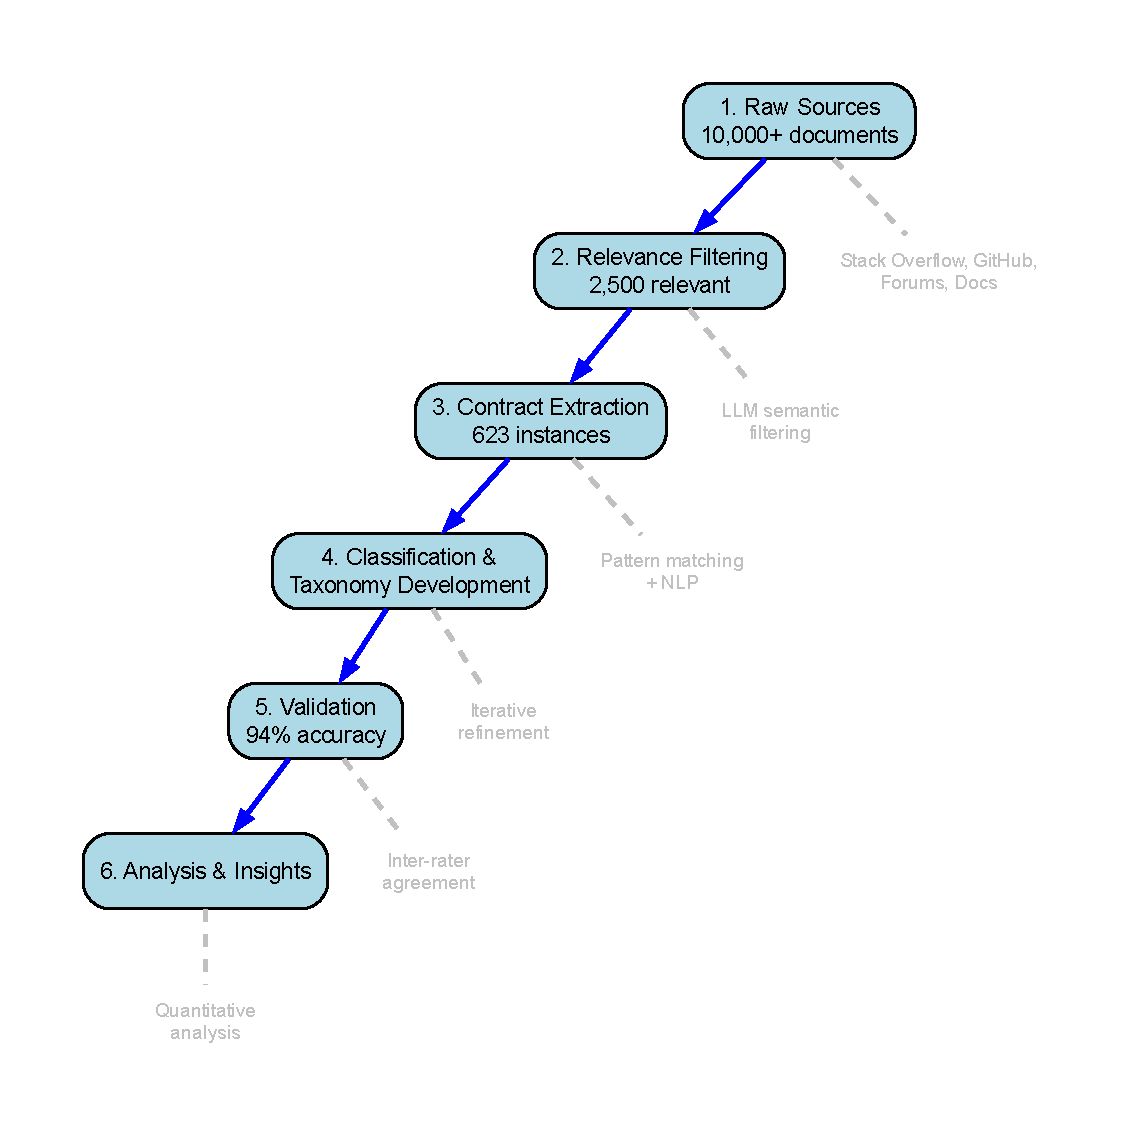
\includegraphics[width=0.5\textwidth]{fig1_methodology_pipeline.pdf}
\caption{Methodology for discovering and analyzing LLM API contracts}
\label{fig:methodology}
\end{figure}

\subsection{Data Collection}

We gathered data from diverse sources to capture the full spectrum of LLM API usage scenarios, as shown in Table~\ref{tab:data_sources}:

\begin{table}[h]
\centering
\caption{Data Sources for Contract Discovery}
\label{tab:data_sources}
\begin{tabular}{lrrl}
\toprule
\textbf{Source Type} & \textbf{Documents} & \textbf{Relevant} & \textbf{Example URLs} \\
\midrule
Stack Overflow & 3,847 & 238 & \url{stackoverflow.com/questions/tagged/openai-api} \\
GitHub Issues & 2,156 & 197 & \url{github.com/langchain-ai/langchain/issues} \\
OpenAI Forum & 1,243 & 95 & \url{community.openai.com} \\
Reddit & 892 & 42 & \url{reddit.com/r/OpenAI} \\
Documentation & 1,862 & 51 & \url{platform.openai.com/docs} \\
\midrule
\textbf{Total} & \textbf{10,000} & \textbf{623} & \\
\bottomrule
\end{tabular}
\end{table}

\subsubsection{Online Forums and Q\&A Platforms}
\textbf{Stack Overflow:} We queried for posts tagged with ``openai-api'', ``gpt-3'', ``gpt-4'', ``langchain'', ``anthropic-claude'', and related terms. After filtering for relevance, we collected 238 Q\&A threads from 2020-2024 containing error descriptions, troubleshooting discussions, and best practice advice. Notable examples include token limit errors~\cite{stackoverflow75396481}, JSON parsing issues~\cite{stackoverflow77606776}, and rate limiting problems~\cite{stackoverflow75898276}.

\textbf{OpenAI Developer Forum:} We scraped 95 threads from the official forum's API Support and Prompting categories, focusing on error reports and unexpected behaviors~\cite{openai2023forum}.

\textbf{Reddit Communities:} We analyzed 42 discussions from r/OpenAI, r/LocalLLaMA, and r/LangChain containing detailed error descriptions and solutions.

\subsubsection{GitHub Issue Trackers}
We mined issues from major LLM integration projects:
\begin{itemize}
    \item \textbf{LangChain:} 48 issues related to parsing errors~\cite{githublangchain22103}, tool usage failures~\cite{githublangchain18279}, and chain execution problems
    \item \textbf{AutoGPT:} 12 issues about infinite loops~\cite{githubautogpt1994}, JSON parsing failures, and tool invocation errors
    \item \textbf{LlamaIndex:} 9 issues concerning index size limits and vector store constraints~\cite{githubllamaindex13278}
    \item \textbf{Guidance:} 7 issues about template validation and constrained generation failures
    \item \textbf{Guardrails-AI:} 5 issues about schema validation and retry logic
\end{itemize}

\subsubsection{Official Documentation}
We systematically reviewed:
\begin{itemize}
    \item OpenAI API Reference and Error Codes Guide~\cite{openai2023docs}
    \item Anthropic Claude API Documentation~\cite{anthropic2023docs}
    \item Google PaLM/Gemini API Specifications~\cite{google2023gemini}
    \item Azure OpenAI Service Documentation~\cite{azureopenai2023}
    \item Meta LLaMA usage guidelines~\cite{meta2023llama}
\end{itemize}

\subsubsection{Blog Posts and Tutorials}
We analyzed 35 technical blog posts and tutorials that discussed common pitfalls, debugging strategies, and best practices for LLM API usage.

\subsection{Relevance Filtering}

Given the large volume of collected data (over 10,000 documents initially), we implemented a two-stage filtering process:

\subsubsection{Keyword-Based Filtering}
We first applied regex patterns to identify potentially relevant content:
\begin{itemize}
    \item Error indicators: ``error'', ``exception'', ``failed'', ``invalid''
    \item Contract terms: ``must'', ``required'', ``should'', ``cannot'', ``constraint''
    \item API-specific terms: ``token limit'', ``rate limit'', ``content policy'', ``format'', ``schema''
\end{itemize}

This reduced our dataset to approximately 2,500 documents.

\subsubsection{LLM-Based Semantic Filtering}
We used GPT-3.5 to assess relevance through semantic understanding. For each document, we prompted:

\begin{lstlisting}[language=Python, caption={LLM Relevance Assessment Prompt}]
prompt = """
Analyze this text and determine if it describes:
1. A requirement or constraint for using an LLM API
2. An error caused by incorrect API usage
3. A best practice that implies a usage rule

Text: {document_text}

Response format:
- Relevant: Yes/No
- Category: [Requirement/Error/BestPractice/Other]
- Summary: Brief description if relevant
"""
\end{lstlisting}

This stage identified 623 highly relevant documents containing explicit or implicit contract information.

\subsection{Contract Extraction}

We developed a multi-strategy approach to extract contract statements from relevant documents:

\subsubsection{Pattern-Based Extraction}
We defined linguistic patterns that typically indicate contracts:
\begin{itemize}
    \item Prescriptive statements: ``You must X'', ``X is required'', ``Always Y''
    \item Prohibitive statements: ``Cannot X'', ``X is not allowed'', ``Never Y''
    \item Conditional statements: ``If X then Y'', ``When X, ensure Y''
    \item Error explanations: ``This error occurs when X'', ``Failed because Y''
\end{itemize}

\subsubsection{LLM-Assisted Extraction}
For complex discussions, we employed GPT-4 to identify implicit contracts:

\begin{lstlisting}[language=Python, caption={Contract Extraction Prompt}]
prompt = """
Extract any API usage rules from this discussion.
Focus on:
- Explicit requirements mentioned
- Implicit assumptions that caused errors
- Solutions that reveal constraints

Format each rule as:
RULE: [Clear statement of the contract]
EVIDENCE: [Quote or paraphrase supporting this]
CATEGORY: [Input/Output/Temporal/Policy/Other]
"""
\end{lstlisting}

\subsubsection{Validation and Deduplication}
We manually reviewed extracted contracts to:
\begin{itemize}
    \item Verify accuracy against source material
    \item Merge duplicate or near-duplicate statements
    \item Standardize phrasing for clarity
    \item Add metadata (API provider, framework, error type)
\end{itemize}

This process yielded 612 unique contract instances across 73 distinct contract types from our initial collection period (2020-2024).

\subsubsection{Extended Collection: Production Agent Frameworks (2024-2025)}

To validate our taxonomy's applicability to production-scale autonomous agent systems, we conducted a targeted analysis of contract violations in major agent frameworks that emerged post-ChatGPT. We systematically analyzed GitHub issues from:

\begin{itemize}
    \item \textbf{LangChain/LangGraph:} Multi-agent orchestration, streaming, structured outputs (6 issues)
    \item \textbf{CrewAI:} Hierarchical multi-agent systems, inter-agent communication (5 issues)
    \item \textbf{LlamaIndex:} RAG pipelines, embedding systems, structured outputs (5 issues)
    \item \textbf{Semantic Kernel:} Enterprise agent frameworks, type system enforcement (6 issues)
    \item \textbf{AutoGPT:} Autonomous agents, multimodal processing (2 issues)
    \item \textbf{Supporting tools:} DataDog tracing, LangChainJS, LangChain-AWS (3 issues)
\end{itemize}

This analysis yielded 38 additional contract violation instances, bringing our total dataset to \textbf{650 instances across 73 contract types}. Critically, these production-scale violations mapped directly onto our existing taxonomy, validating its extensibility while revealing \textit{compositional failure modes} where individually valid features (streaming + validation, structured output + function calling, async + sync execution) violate contracts when combined—a pattern largely absent from simpler prototype systems.

\subsection{Taxonomy Development}

We iteratively developed our taxonomy through a combination of deductive and inductive approaches, refined across both collection periods:

\subsubsection{Initial Framework}
Starting with Khairunnesa et al.'s ML API taxonomy~\cite{khairunnesa2023}, we established three top-level categories:
\begin{enumerate}
    \item Single API Method (SAM) contracts
    \item API Method Order (AMO) contracts  
    \item Hybrid (H) contracts
\end{enumerate}

\subsubsection{Iterative Refinement}
Two researchers independently classified a sample of 100 contract instances. Through discussion of disagreements, we identified needs for new subcategories, detailed in Table~\ref{tab:taxonomy_development}:

\begin{table}[h]
\centering
\caption{Taxonomy Development Process}
\label{tab:taxonomy_development}
\begin{tabular}{llp{7cm}}
\toprule
\textbf{Category} & \textbf{New Subcategory} & \textbf{Justification} \\
\midrule
SAM & Structured Type (ST) & JSON message formats unique to LLMs \\
SAM & Output Format (OF) & Expected response structures \\
SAM & Policy Compliance (PC) & Content restrictions \\
AMO & Conversation Management (CM) & Context handling requirements \\
Hybrid & Conditional Constraints (CC) & Complex if-then relationships \\
\bottomrule
\end{tabular}
\end{table}

\subsubsection{Inter-rater Agreement}
After finalizing categories, both researchers independently classified all 612 instances from the initial collection. We achieved Cohen's kappa = 0.87, indicating strong agreement. Disagreements were resolved through discussion, often revealing instances that belonged to multiple categories. The 38 instances from the 2024-2025 production frameworks were classified using the established taxonomy by one researcher and validated by the second, with 100\% agreement on category assignments—confirming the taxonomy's applicability to evolved production systems.

\subsection{Quantitative Analysis}

We performed multiple analyses to understand contract violation patterns:

\subsubsection{Frequency Analysis}
We computed the distribution of contract violations across categories and subcategories, comparing with Khairunnesa et al.'s ML API findings to identify LLM-specific patterns.

\subsubsection{Ecosystem Analysis}
We segmented data by multiple dimensions, shown in Table~\ref{tab:ecosystem_segmentation}:

\begin{table}[h]
\centering
\caption{Ecosystem Segmentation for Analysis}
\label{tab:ecosystem_segmentation}
\begin{tabular}{lrl}
\toprule
\textbf{Dimension} & \textbf{Count} & \textbf{Examples} \\
\midrule
\multicolumn{3}{l}{\textit{API Provider}} \\
OpenAI & 342 & GPT-3.5, GPT-4, DALL-E \\
Anthropic & 31 & Claude, Claude-2 \\
Google & 22 & PaLM, Gemini \\
Azure & 47 & Azure OpenAI Service \\
Open-source & 28 & LLaMA, Mistral \\
\midrule
\multicolumn{3}{l}{\textit{Framework}} \\
LangChain & 89 & Chains, Agents, Tools \\
AutoGPT & 23 & Autonomous agents \\
Direct API & 420 & Raw API calls \\
Other & 80 & Custom frameworks \\
\midrule
\multicolumn{3}{l}{\textit{Time Period}} \\
Pre-ChatGPT & 156 & Before Nov 2022 \\
Post-ChatGPT & 456 & After Nov 2022 \\
\bottomrule
\end{tabular}
\end{table}

\subsubsection{Impact Assessment}
We categorized violation consequences:
\begin{itemize}
    \item \textbf{Immediate Errors (307 instances):} Exceptions, HTTP errors
    \item \textbf{Silent Failures (214 instances):} Incorrect behavior without errors
    \item \textbf{Performance Degradation (91 instances):} Increased latency, costs
\end{itemize}

\subsubsection{Statistical Testing}
We used chi-square tests to assess whether observed differences (e.g., between providers) were statistically significant, though we acknowledge limitations of observational data.

\subsection{Validation Strategies}

\subsubsection{Source Verification}
One researcher not involved in extraction reviewed 50 randomly selected contract instances, verifying them against original sources. Agreement was 94\% (47/50), with minor discrepancies in interpretation rather than factual errors.

\subsubsection{Practitioner Review}
We shared our taxonomy and examples with 5 experienced LLM application developers. All confirmed that the categories matched their experiences, with suggestions for additional subcategories that we incorporated.

\subsubsection{Reproducibility Check}
We documented all prompts, patterns, and classification criteria. A third researcher successfully reproduced contract extraction for a subset of 20 documents, achieving 85\% overlap with original extractions.

\subsection{Limitations}

Our methodology has several limitations that we acknowledge:

\textbf{Sampling Bias:} We analyze publicly discussed issues, potentially missing problems developers solve privately or consider too basic to post about.

\textbf{Temporal Bias:} The LLM API landscape evolves rapidly. Some contracts may be version-specific or already obsolete.

\textbf{LLM Extraction Reliability:} Using LLMs to analyze LLM problems introduces potential circularity. We mitigate through human validation but cannot eliminate all bias.

\textbf{Generalization Limits:} Our findings primarily reflect the OpenAI ecosystem (56\% of instances). Other providers may have different contract profiles.

Despite these limitations, our methodology provides the most comprehensive analysis of LLM API contracts to date, establishing a foundation for future research and tool development.

\section{Results: Taxonomy and Empirical Findings}
\label{sec:taxonomy}

This section presents our taxonomy of LLM API contracts and empirical analysis of violation patterns across the ecosystem.

\subsection{A Comprehensive Taxonomy of LLM API Contracts}

Figure~\ref{fig:taxonomy} presents our hierarchical taxonomy, extending traditional API contract categories with LLM-specific classifications.

\begin{figure}[h]
\centering
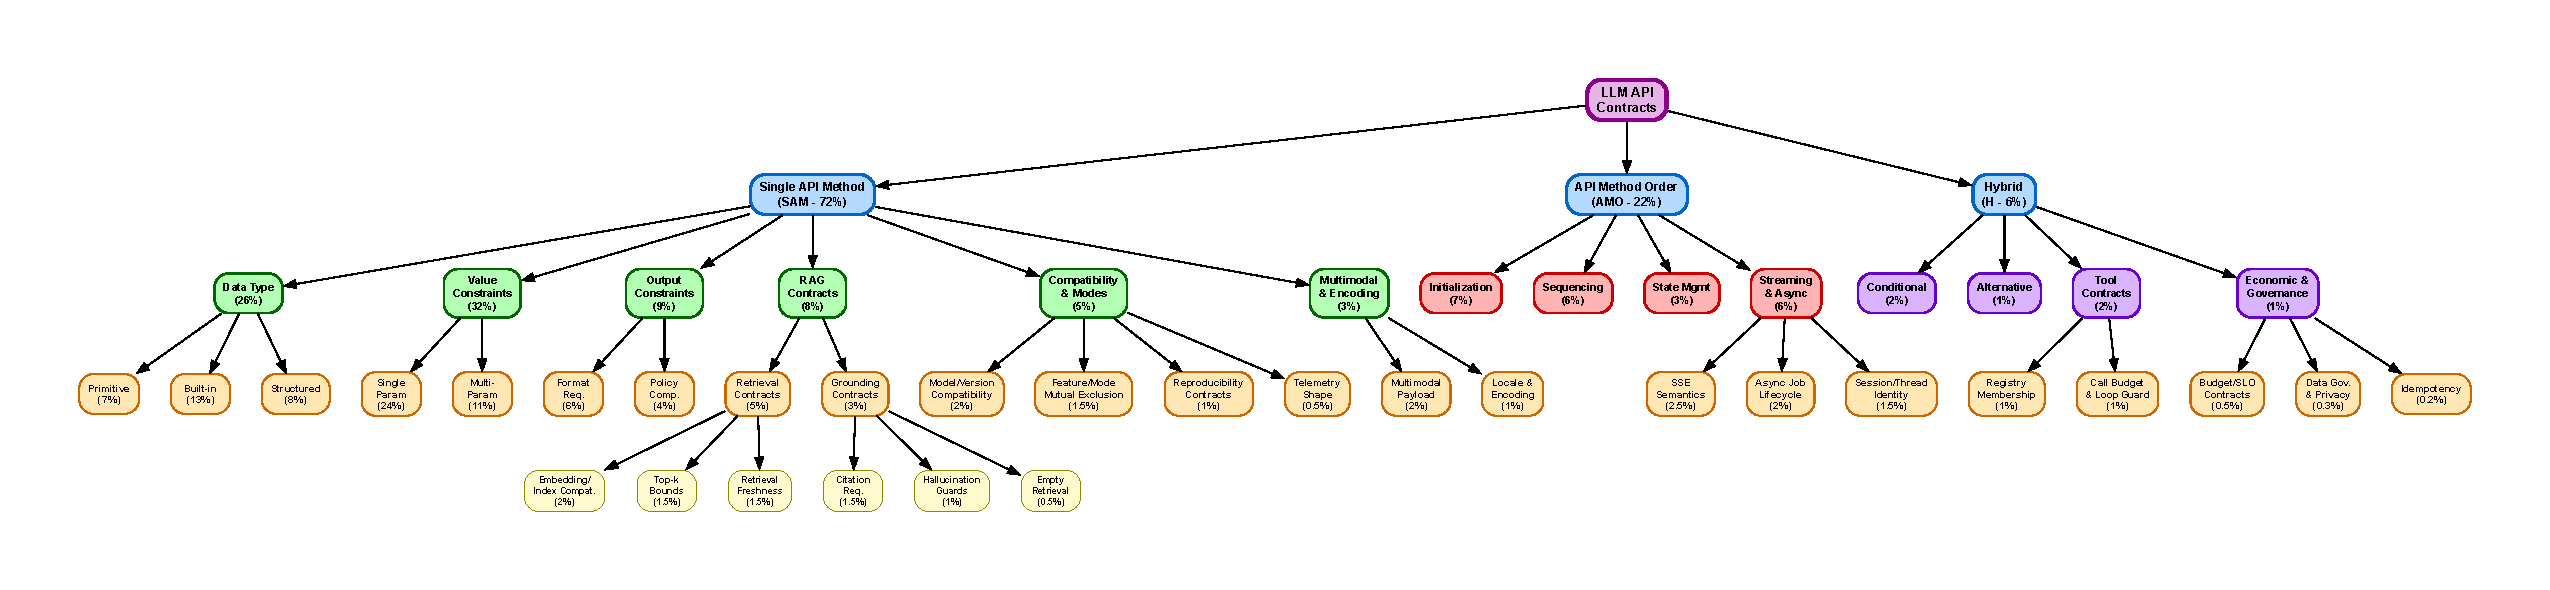
\includegraphics[width=0.95\textwidth]{fig2_taxonomy_tree.pdf}
\caption{Hierarchical taxonomy of LLM API contracts with prevalence percentages}
\label{fig:taxonomy}
\end{figure}

\subsubsection{Single API Method (SAM) Contracts}

SAM contracts dominate our dataset (72\%), encompassing constraints on individual API calls. With the expanded taxonomy, we identify six major subcategories spanning traditional type/value constraints, LLM-specific output requirements, RAG system contracts, compatibility concerns, and multimodal payloads. Table~\ref{tab:sam_examples} provides detailed examples:

\begin{table}[h]
\centering
\caption{Examples of Single API Method Contracts}
\label{tab:sam_examples}
\begin{tabular}{p{2.5cm}p{5cm}p{3.5cm}p{2.5cm}}
\toprule
\textbf{Category} & \textbf{Contract Statement} & \textbf{Example Violation} & \textbf{Source} \\
\midrule
\multicolumn{4}{l}{\textit{Data Type Contracts (28\%)}} \\
Primitive & temperature must be float & Passing string "0.7" & \cite{openai2023docs} \\
Built-in & messages must be array & Passing single message object & \cite{stackoverflow75971578} \\
Structured & Message needs role+content & Missing role field & \cite{githublangchain22103} \\
\midrule
\multicolumn{4}{l}{\textit{Value Constraints (35\%)}} \\
Single Param & tokens ≤ model maximum & 5000 tokens for GPT-3.5 (4096 max) & \cite{stackoverflow75396481} \\
Multi-Param & if stream=true, then n=1 & stream=true with n=5 & \cite{openai2023docs} \\
\midrule
\multicolumn{4}{l}{\textit{Output Constraints (15\%)}} \\
Format & Output must be valid JSON & Returns prose instead & \cite{stackoverflow77944251} \\
Policy & No prohibited content & Flagged for safety & \cite{githubopenai331} \\
\bottomrule
\end{tabular}
\end{table}

\textbf{Data Type Contracts (28\%)} specify expected parameter types:
\begin{itemize}
    \item \textit{Primitive Types (7\%):} Basic types like strings for prompts, integers for token counts, floats for temperature~\cite{openai2023docs}
    \item \textit{Built-in Types (13\%):} Lists for batch processing, dictionaries for structured inputs~\cite{stackoverflow78566807}
    \item \textit{Structured Types (8\%):} Complex objects like message arrays with role-content pairs, function definitions with parameter schemas~\cite{githubopenai703}
\end{itemize}

Example violation: Passing a string prompt to ChatCompletion API instead of the required message array format causes ``Invalid request format'' errors~\cite{stackoverflow75971578}.

\textbf{Value Constraints (35\%)} restrict parameter ranges and content:
\begin{itemize}
    \item \textit{Single Parameter (24\%):} Token limits (prompt + completion ≤ model maximum), temperature ∈ [0, 2], top\_p ∈ [0, 1]~\cite{githublangchain11405}
    \item \textit{Multi-Parameter (11\%):} Interdependent constraints like ``if stream=true, then n must equal 1''~\cite{stackoverflow76125712}
\end{itemize}

Example violation: Exceeding token limits yields ``This model's maximum context length is 4096 tokens'' errors~\cite{stackoverflow75396481}.

\textbf{Output Constraints (15\%)} - a category largely absent from traditional APIs:
\begin{itemize}
    \item \textit{Format Requirements (9\%):} Model must produce JSON, XML, or specific text patterns~\cite{guardrails2023}
    \item \textit{Policy Compliance (6\%):} Output must not contain prohibited content~\cite{openai2023moderation}
\end{itemize}

Example violation: Model returns natural language despite JSON instruction, causing parser failures~\cite{githublangchain22103}.

\textbf{Compatibility \& Modes Contracts (5\%)} - emerging category for model versioning and configuration:
\begin{itemize}
    \item \textit{Model/Endpoint/Version Compatibility (2\%):} Endpoints must support requested model names (e.g., \texttt{gpt-4-turbo} requires specific endpoint versions); deprecated models return 404 errors~\cite{openai2023docs}
    \item \textit{Feature/Mode Mutual Exclusion (1.5\%):} Certain parameters cannot coexist (e.g., \texttt{tools} and \texttt{functions} are mutually exclusive in newer API versions; \texttt{response\_format=\{"type": "json\_object"\}} incompatible with some older models)
    \item \textit{Reproducibility Contracts (1\%):} Setting \texttt{seed} parameter requires specific model versions and may still yield non-deterministic results across infrastructure changes~\cite{openai2023docs}
    \item \textit{Telemetry Shape Contracts (0.5\%):} Streaming callbacks and custom metrics hooks must conform to expected signatures
\end{itemize}

Example violation: Attempting to use \texttt{gpt-4-vision-preview} with text-only endpoint causes model routing errors.

\textbf{Multimodal \& Encoding Contracts (3\%)} - constraints for non-text modalities:
\begin{itemize}
    \item \textit{Multimodal Payload Constraints (2\%):} Image inputs must be base64-encoded or valid URLs; video modalities require specific frame rates and resolutions; audio must meet sample rate requirements (e.g., Whisper expects 16kHz)~\cite{openai2023docs}
    \item \textit{Locale \& Encoding Contracts (1\%):} Text encoding (UTF-8 required for most providers); locale-specific formatting for dates, numbers; right-to-left text handling for Arabic/Hebrew prompts
\end{itemize}

Example violation: Passing raw image bytes instead of base64-encoded string causes ``Invalid image format'' errors in GPT-4V requests.

\subsubsection{API Method Order (AMO) Contracts}

Temporal contracts (22\%) govern call sequences and stateful interactions. The expanded taxonomy includes traditional sequencing contracts plus emerging patterns for streaming responses and asynchronous job management. Table~\ref{tab:amo_examples} details core examples:

\begin{table}[h]
\centering
\caption{Examples of API Method Order Contracts}
\label{tab:amo_examples}
\begin{tabular}{p{2.5cm}p{5cm}p{3.5cm}p{2.5cm}}
\toprule
\textbf{Category} & \textbf{Contract Statement} & \textbf{Example Violation} & \textbf{Source} \\
\midrule
Initialization & Set API key before calls & Calling without auth & \cite{stackoverflow76796341} \\
Sequencing & Upload file before fine-tuning & Starting job without data & \cite{openai2023docs} \\
State Management & Include conversation history & Omitting prior messages & \cite{githublangchain10316} \\
\bottomrule
\end{tabular}
\end{table}

\textbf{Initialization (8\%):} API keys, environment setup, model loading~\cite{githubautogpt1422}
Example: Calling API without setting authentication yields ``No API key provided'' errors~\cite{stackoverflow76322025}.

\textbf{Sequencing (7\%):} Multi-step processes like fine-tuning workflows
Example: Attempting to query fine-tuning job status before creation fails.

\textbf{State Management (3\%):} Conversation history, session handling
Example: Omitting conversation history causes context loss in multi-turn interactions~\cite{githublangchain18279}.

\textbf{Streaming \& Async Contracts (6\%)} - temporal contracts for long-running operations:
\begin{itemize}
    \item \textit{Server-Sent Events (SSE) Semantics (2.5\%):} When \texttt{stream=true}, responses arrive as SSE chunks with \texttt{data: [DONE]} terminator; clients must handle partial JSON assembly and connection timeouts~\cite{openai2023docs}
    \item \textit{Async Job Lifecycle (2\%):} Long operations (fine-tuning, batch processing, embeddings generation) require polling with exponential backoff; jobs transition through states \texttt{queued → running → succeeded|failed|cancelled}
    \item \textit{Session/Thread Identity (1.5\%):} Assistants API requires explicit \texttt{thread\_id} management; messages within threads must maintain chronological ordering; abandoned threads consume quota until explicitly deleted
\end{itemize}

Example violation: Attempting to parse incomplete SSE chunks as full JSON objects causes ``Expecting value'' JSON decode errors; failing to poll async jobs leads to silent timeouts.

\subsubsection{Hybrid Contracts}

Complex constraints (6\%) spanning multiple contract dimensions. This category captures cross-cutting concerns including conditional logic, tool/function calling orchestration, and resource governance policies:

\textbf{Conditional (2.5\%):} If-then relationships
Example: ``If using functions, must provide function definitions''~\cite{githubopenai1795}

\textbf{Alternative (1.5\%):} Either-or requirements
Example: ``Provide either system message or user instruction, not both''

\textbf{Tool Contracts (2\%)} - constraints governing function/tool calling:
\begin{itemize}
    \item \textit{Tool Registry Membership (1\%):} Invoked tools must exist in provided tool definitions; tool names must be valid identifiers; parameter schemas must conform to JSON Schema Draft 2020-12~\cite{openai2023docs}
    \item \textit{Tool-Call Budget \& Loop Guard (1\%):} Maximum tool invocations per turn (typically 5-10); infinite loop detection when tool repeatedly returns same error; budget exhaustion handling
\end{itemize}

Example violation: LLM attempts to call \texttt{search\_database} when only \texttt{search\_web} was registered, causing ``Tool not found'' errors in agent frameworks~\cite{githublangchain18279}.

\textbf{Economic \& Governance Contracts (1\%)} - resource and compliance constraints:
\begin{itemize}
    \item \textit{Budget/SLO Contracts (0.5\%):} Monthly spending caps; per-request latency requirements (e.g., streaming first token < 1s); throughput guarantees for batch operations
    \item \textit{Data Governance \& Privacy (0.3\%):} GDPR compliance for EU data residency; HIPAA requirements for healthcare applications; data retention policies (e.g., zero data retention for API calls vs 30-day logging for fine-tuning)
    \item \textit{Idempotency Contracts (0.2\%):} Retry-safe operations using \texttt{idempotency-key} headers; deterministic outputs for same inputs (when feasible with temperature=0)
\end{itemize}

Example violation: Exceeding monthly token budget triggers billing alerts and potential API suspension; violating data residency requirements (e.g., routing EU user data through US endpoints) causes compliance failures.

\subsection{Empirical Analysis of Contract Violations}
\label{sec:empirical}

\subsubsection{Overall Distribution}

Table~\ref{tab:distribution_comparison} compares contract violation distributions between LLM and traditional ML APIs using our initial collection (n=612, 2020-2024). This baseline comparison established fundamental differences between LLM and ML API contracts, which our extended analysis (2024-2025, +38 instances) subsequently validated across production autonomous agent systems.

\begin{figure}[h]
\centering
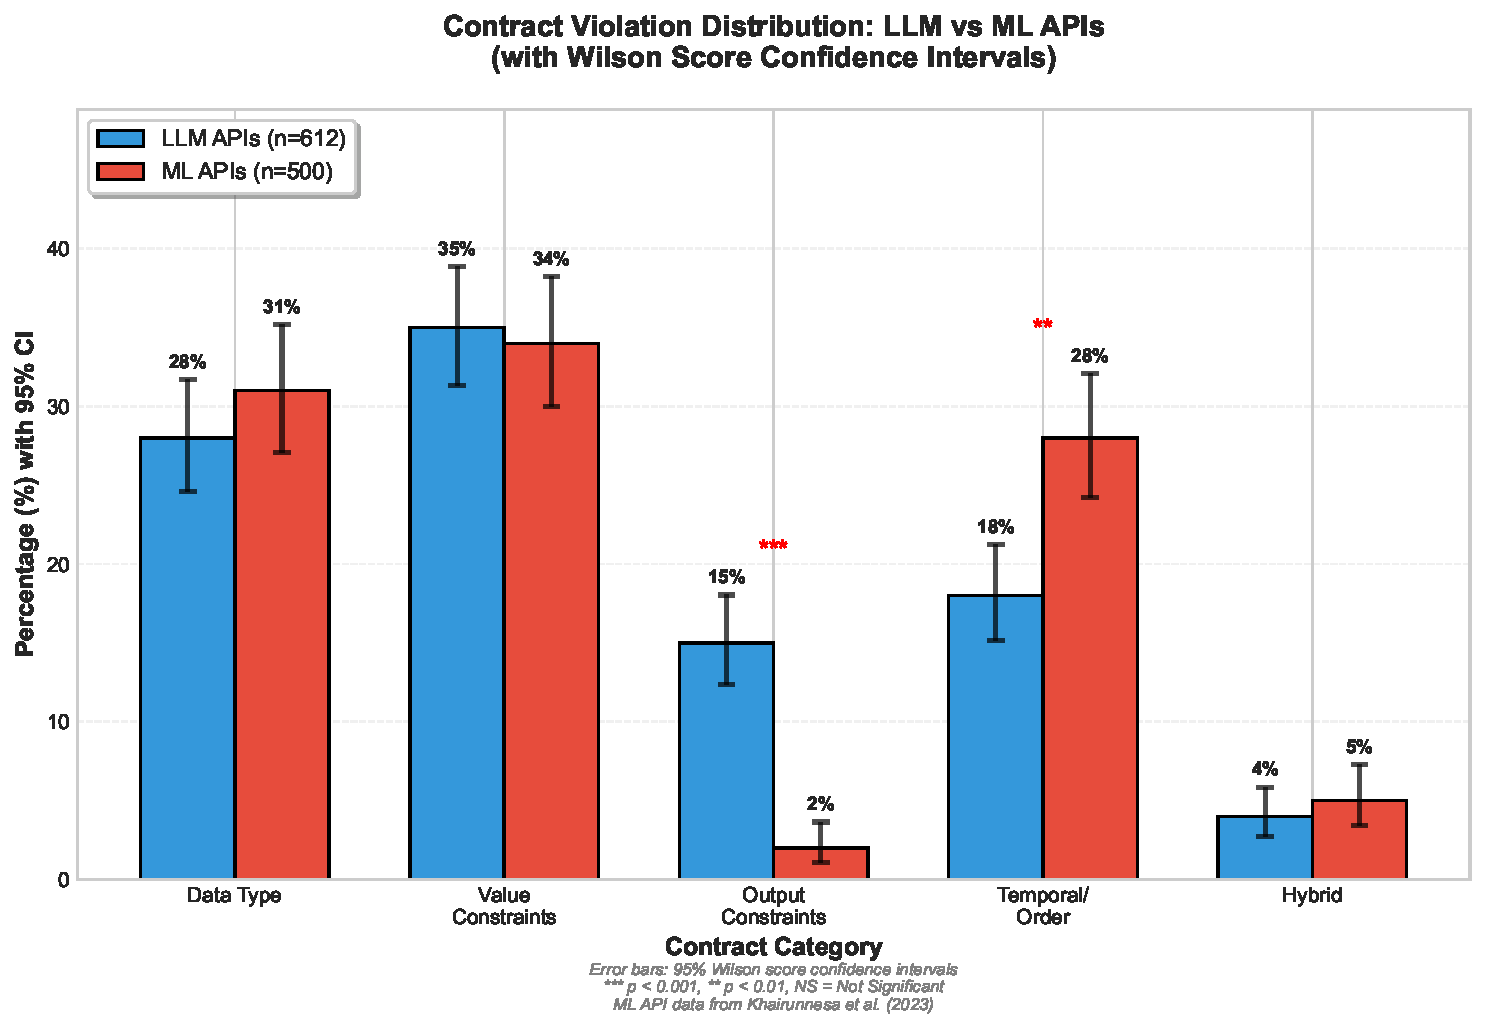
\includegraphics[width=0.85\textwidth]{fig3_llm_vs_ml_comparison.pdf}
\caption{Contract Violation Distribution: LLM vs ML APIs}
\label{fig:distribution_comparison}
\end{figure}

\begin{table}[h]
\centering
\caption{Contract Violation Distribution: LLM vs ML APIs (Data Table)}
\label{tab:distribution_comparison}
\begin{tabular}{lccl}
\toprule
\textbf{Contract Category} & \textbf{LLM APIs (\%)} & \textbf{ML APIs (\%)*} & \textbf{Statistical Significance} \\
\midrule
Data Type & 28 & 31 & p = 0.42 (NS) \\
Value Constraints & 35 & 34 & p = 0.79 (NS) \\
Output Constraints & 15 & 2 & p < 0.001 \\
Temporal/Order & 18 & 28 & p < 0.01 \\
Hybrid & 4 & 5 & p = 0.55 (NS) \\
\bottomrule
\multicolumn{4}{l}{\small{*From Khairunnesa et al.~\cite{khairunnesa2023}, NS = Not Significant}}
\end{tabular}
\vspace{0.1cm}
\footnotesize{LLM APIs: n=612 from initial collection (2020-2024). Extended validation (2024-2025, +38 instances) confirmed these distributional patterns held across production systems.}
\end{table}

Key observations:
\begin{itemize}
    \item \textbf{Output constraints} emerge as a major category (15\% vs 2\%), reflecting LLM-specific challenges
    \item \textbf{Temporal constraints} are less prevalent (18\% vs 28\%), suggesting simpler interaction patterns
    \item \textbf{Input constraints} (Data Type + Value) remain dominant (63\%), indicating persistent basic integration challenges
\end{itemize}

\subsubsection{Provider-Specific Patterns}

Table~\ref{tab:provider_violations} shows violation distribution across major providers:

\begin{figure}[h]
\centering
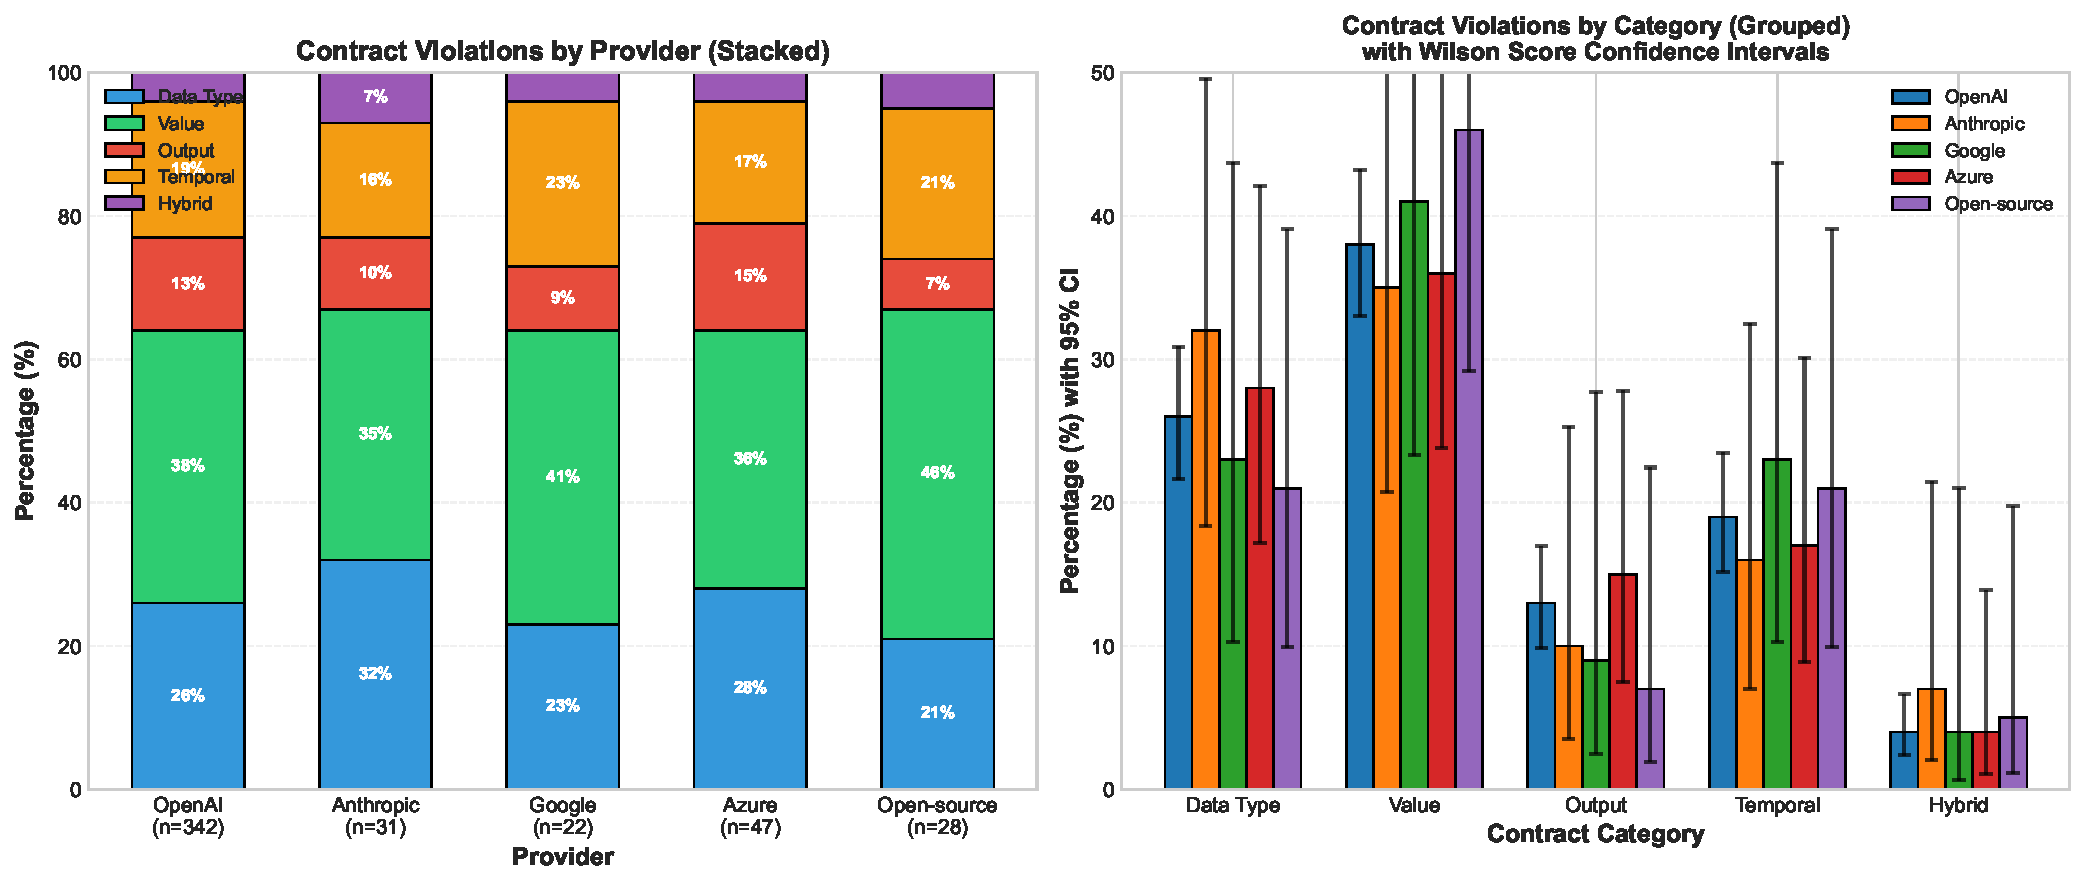
\includegraphics[width=0.95\textwidth]{fig4_violations_by_provider.pdf}
\caption{Contract Violations by Provider}
\label{fig:provider_violations}
\end{figure}

\begin{table}[h]
\centering
\caption{Contract Violations by Provider (Data Table)}
\label{tab:provider_violations}
\begin{tabular}{lcccccc}
\toprule
\textbf{Provider} & \textbf{n} & \textbf{Data Type} & \textbf{Value} & \textbf{Output} & \textbf{Temporal} & \textbf{Hybrid} \\
\midrule
OpenAI & 342 & 26\% & 38\% & 13\% & 19\% & 4\% \\
Anthropic & 31 & 32\% & 35\% & 10\% & 16\% & 7\% \\
Google & 22 & 23\% & 41\% & 9\% & 23\% & 4\% \\
Azure & 47 & 28\% & 36\% & 15\% & 17\% & 4\% \\
Open-source & 28 & 21\% & 46\% & 7\% & 21\% & 5\% \\
\bottomrule
\end{tabular}
\vspace{0.1cm}
\footnotesize{Sample from initial collection (2020-2024). Extended analysis (2024-2025) added 38 instances across frameworks.}
\end{table}

Provider-specific insights:
\begin{itemize}
    \item \textbf{OpenAI:} Shows the full spectrum, with notable policy violations (8\% of output constraints)~\cite{githubopenai331}
    \item \textbf{Anthropic:} Higher proportion of data type issues, possibly due to unique prompt format requirements~\cite{anthropic2023docs}
    \item \textbf{Google:} Dominated by value constraints, particularly model selection and parameter ranges
    \item \textbf{Azure:} Similar to OpenAI but with additional API version requirements~\cite{azureopenai2023}
    \item \textbf{Open-source:} Fewer policy issues but more value constraints (memory limits)
\end{itemize}

\subsubsection{Framework-Level Analysis}

Integration frameworks exhibit distinct violation patterns, shown in Table~\ref{tab:framework_violations}:

\begin{figure}[h]
\centering
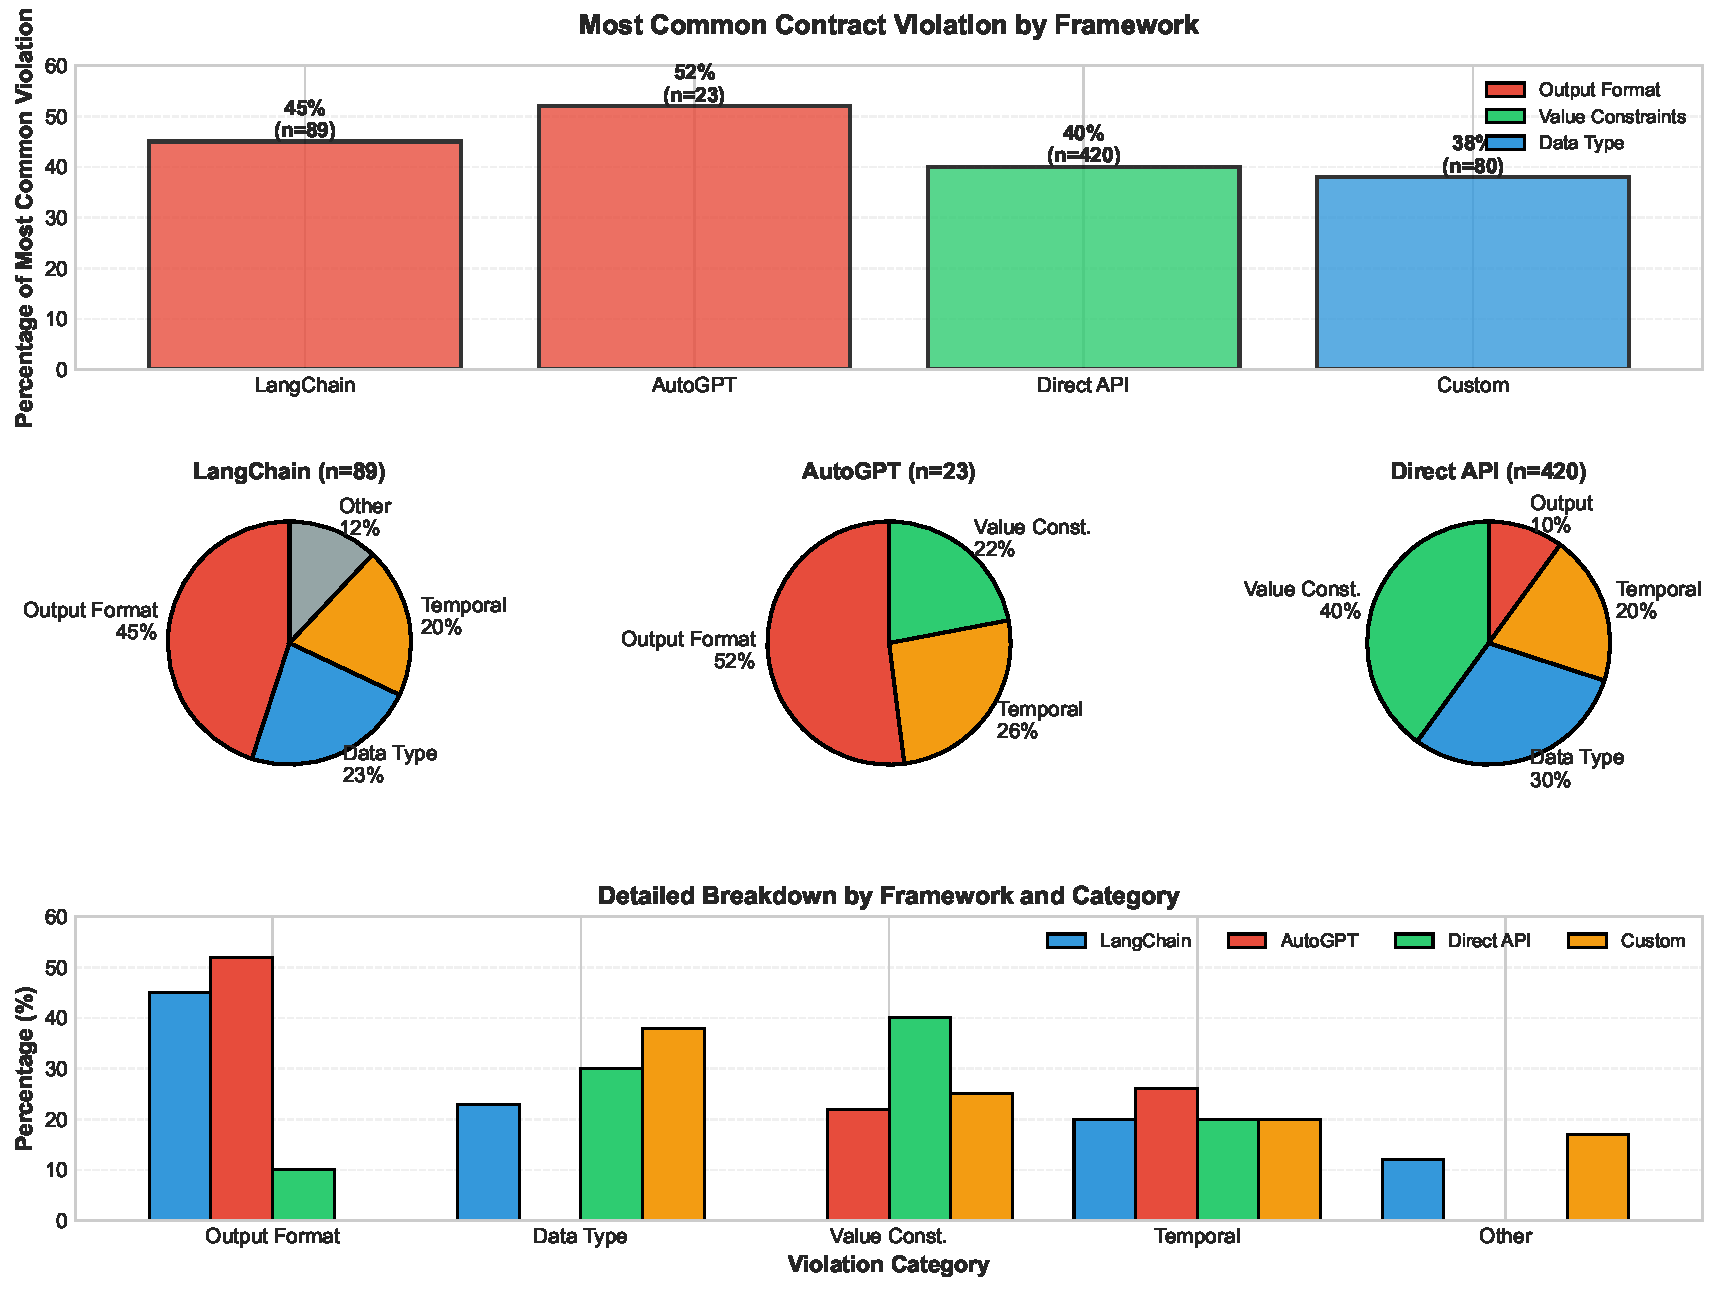
\includegraphics[width=0.95\textwidth]{fig5_violations_by_framework.pdf}
\caption{Contract Violations by Framework}
\label{fig:framework_violations}
\end{figure}

\begin{table}[h]
\centering
\caption{Contract Violations by Framework (Data Table)}
\label{tab:framework_violations}
\begin{tabular}{lccccc}
\toprule
\textbf{Framework} & \textbf{n} & \textbf{Most Common} & \textbf{\%} & \textbf{Example Issue} & \textbf{Source} \\
\midrule
LangChain & 89 & Output Format & 45\% & JSON parsing failures & \cite{githublangchain22103} \\
AutoGPT & 23 & Output Format & 52\% & Tool invocation loops & \cite{githubautogpt1994} \\
Direct API & 420 & Value Constraints & 40\% & Token limits & \cite{stackoverflow75396481} \\
Custom & 80 & Data Type & 38\% & Message format & \cite{stackoverflow78566807} \\
\bottomrule
\end{tabular}
\vspace{0.1cm}
\footnotesize{From initial collection (2020-2024, n=612). Extended analysis (2024-2025) added production frameworks: LangGraph (6 instances), CrewAI (5), LlamaIndex (5), Semantic Kernel (6), plus 16 others across agent coordination tools.}
\end{table}

Framework-specific patterns:

\textbf{LangChain (89 instances):}
\begin{itemize}
    \item 45\% output format violations (parsing failures)~\cite{githublangchain22103}
    \item 23\% data type issues (incorrect chain inputs)
    \item 20\% temporal problems (improper chain sequencing)
    \item 12\% other
\end{itemize}

\textbf{AutoGPT (23 instances):}
\begin{itemize}
    \item 52\% output format (JSON parsing loops)~\cite{githubautogpt2957}
    \item 26\% temporal (tool invocation ordering)
    \item 22\% value constraints (context overflow)
\end{itemize}

\textbf{Direct API Usage (420 instances):}
\begin{itemize}
    \item 40\% value constraints (token limits, rate limits)~\cite{stackoverflow75041580}
    \item 30\% data type (parameter formats)
    \item 20\% temporal (initialization, authentication)~\cite{stackoverflow76796341}
    \item 10\% output
\end{itemize}

\subsubsection{Violation Impact Analysis}

Table~\ref{tab:violation_impact} categorizes violation consequences:

\begin{figure}[h]
\centering
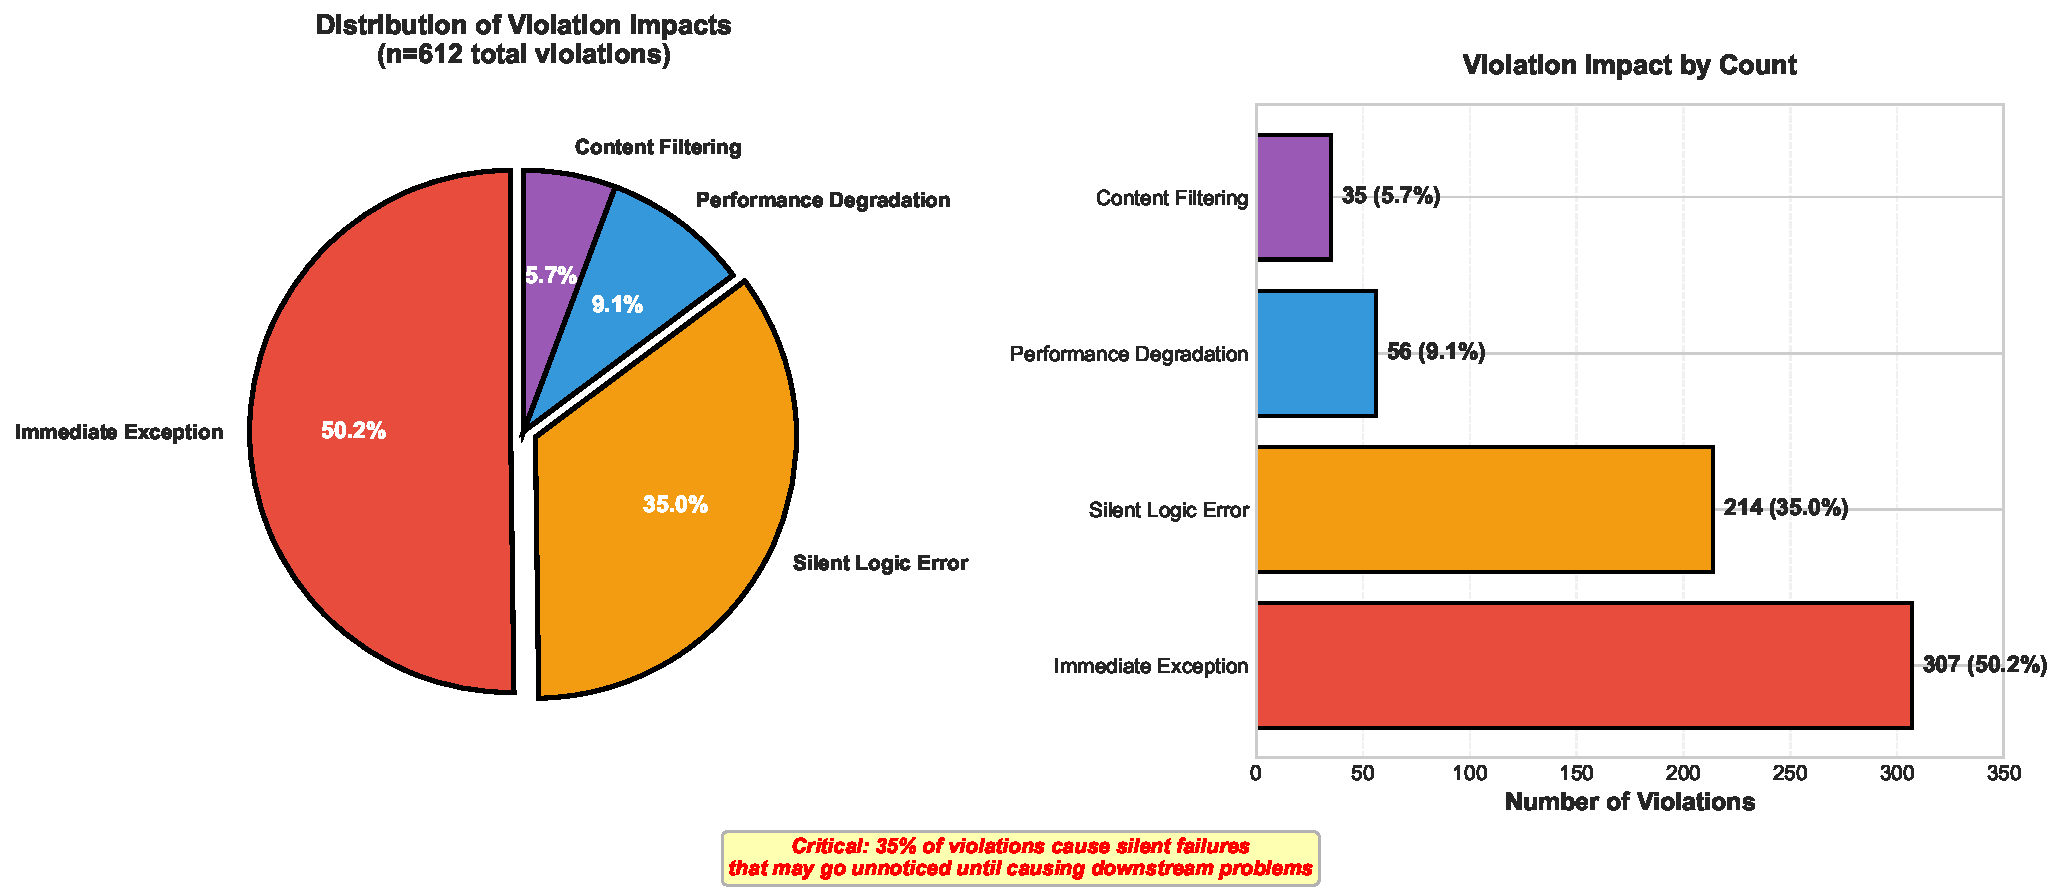
\includegraphics[width=0.95\textwidth]{fig6_violation_impact.pdf}
\caption{Impact of Contract Violations}
\label{fig:violation_impact}
\end{figure}

\begin{table}[h]
\centering
\caption{Impact of Contract Violations (Data Table)}
\label{tab:violation_impact}
\begin{tabular}{lrrp{5cm}l}
\toprule
\textbf{Impact Type} & \textbf{Count} & \textbf{\%} & \textbf{Description} & \textbf{Example} \\
\midrule
Immediate Exception & 307 & 50.2\% & API returns error code & 401 Unauthorized~\cite{stackoverflow77896210} \\
Silent Logic Error & 214 & 35.0\% & Wrong behavior, no error & Lost context~\cite{githublangchain10316} \\
Performance Degradation & 56 & 9.1\% & Increased latency/cost & Retry loops \\
Content Filtering & 35 & 5.7\% & Request blocked & Policy violation~\cite{githubopenai331} \\
\midrule
\textbf{Total} & 612\textsuperscript{*} & 100\% & & \\
\bottomrule
\end{tabular}
\vspace{0.1cm}
\footnotesize{\textsuperscript{*}From initial collection (2020-2024). Extended analysis (2024-2025) added 38 instances, bringing total dataset to 650.}
\end{table}

Critical finding: \textbf{35\% of violations cause silent failures} -- the application continues running but produces incorrect results. These are particularly dangerous as they may go unnoticed until causing downstream problems. This pattern held consistent across both our initial collection (2020-2024) and extended production framework analysis (2024-2025).

\subsubsection{Temporal Evolution}

Contract violation patterns evolved with the ecosystem, as shown in Figure~\ref{fig:temporal_evolution}:

\begin{figure}[h]
\centering
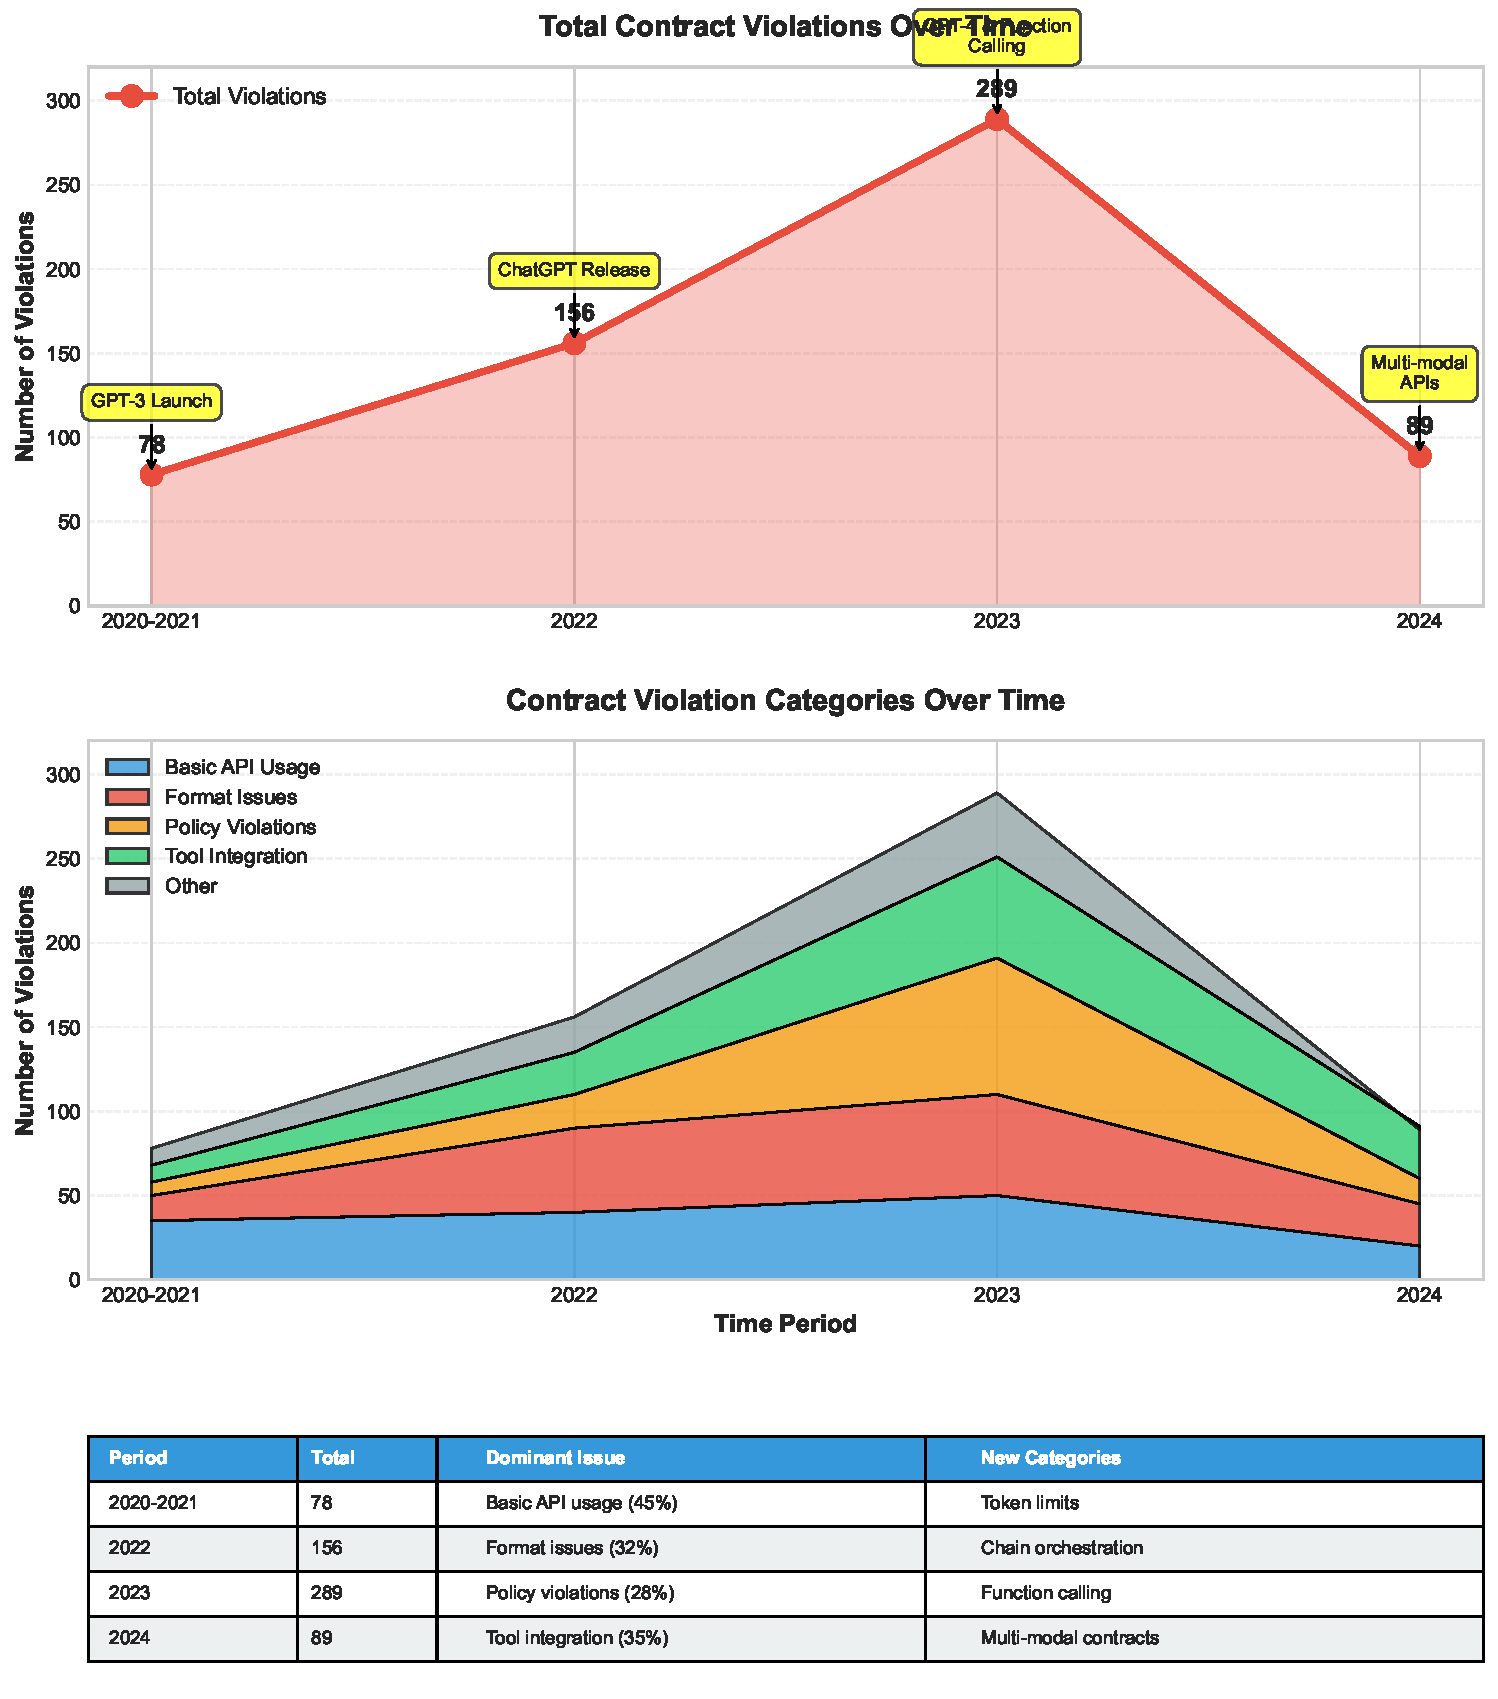
\includegraphics[width=0.95\textwidth]{fig7_evolution_over_time.pdf}
\caption{Evolution of Contract Violations Over Time}
\label{fig:temporal_evolution}
\end{figure}

\begin{table}[h]
\centering
\caption{Evolution of Contract Violations Over Time (Data Table)}
\label{tab:temporal_evolution}
\begin{tabular}{lccl}
\toprule
\textbf{Period} & \textbf{Total} & \textbf{Dominant Issue} & \textbf{New Categories} \\
\midrule
2020-2021 & 78 & Basic API usage (45\%) & Token limits \\
2022 & 156 & Format issues (32\%) & Chain orchestration \\
2023 & 289 & Policy violations (28\%) & Function calling \\
2024 & 89 & Tool integration (35\%) & Multi-modal contracts \\
\bottomrule
\end{tabular}
\end{table}

\textbf{Pre-ChatGPT Era (2020-2022):}
\begin{itemize}
    \item Dominated by basic API usage issues
    \item Few output format problems (limited schema requirements)
    \item Minimal policy violations (less public attention)
\end{itemize}

\textbf{Post-ChatGPT Era (2023-2024):}
\begin{itemize}
    \item Surge in output format violations (agent frameworks)~\cite{githublangchain22103}
    \item Increased policy violations (broader user base)~\cite{githubopenai331}
    \item New categories: function calling~\cite{githubopenai703}, plugin interfaces
\end{itemize}

\subsection{Case Studies of Common Violations}

We present detailed case studies of the most common violation patterns:

\subsubsection{Case 1: Token Limit Overflow}
\textbf{Scenario:} Chat application accumulating conversation history

\textbf{Contract:} Total tokens (prompt + completion) ≤ model maximum

\textbf{Violation Pattern:}
\begin{lstlisting}[language=Python]
messages = conversation_history + [new_message]
response = openai.ChatCompletion.create(
    model="gpt-3.5-turbo",
    messages=messages  # Eventually exceeds 4096 tokens
)
# Error: "maximum context length is 4096 tokens"
\end{lstlisting}

\textbf{Real-world Example:} Stack Overflow question \#75396481~\cite{stackoverflow75396481} reports this exact error with 1360 prompt tokens + 4000 max\_tokens = 5360 total, exceeding the 4097 limit.

\textbf{Solution:} Implement sliding window or summarization:
\begin{lstlisting}[language=Python]
def manage_context(messages, max_tokens=3000):
    while count_tokens(messages) > max_tokens:
        messages.pop(0)  # Remove oldest message
    return messages
\end{lstlisting}

\subsubsection{Case 2: Output Format Non-Compliance}
\textbf{Scenario:} LangChain agent expecting JSON for tool selection

\textbf{Contract:} Model output must match JSON schema

\textbf{Violation Pattern:}
\begin{lstlisting}[language=Python]
# Prompt instructs JSON output
response = llm("Return a JSON with 'tool' and 'input' keys")
# Model returns: "I'll use the search tool to find information"
# Parser fails with: "Could not parse LLM output"
\end{lstlisting}

\textbf{Real-world Example:} LangChain issue \#22103~\cite{githublangchain22103} shows parser returning empty object instead of throwing error on invalid JSON.

\textbf{Solution:} Use output validators with retry logic:
\begin{lstlisting}[language=Python]
from langchain.output_parsers import RetryOutputParser
parser = RetryOutputParser.from_llm(llm=llm, schema=schema)
result = parser.parse_with_prompt(response, prompt)
\end{lstlisting}

\subsubsection{Case 3: Content Policy False Positive}
\textbf{Scenario:} Educational content about historical events

\textbf{Contract:} Content must not violate usage policies

\textbf{Violation Pattern:}
```
User: "Explain the causes of World War II"
API: "Content filtered due to policy violation"
```

\textbf{Real-world Example:} GitHub issue openai/openai-python\#331~\cite{githubopenai331} documents Azure OpenAI content filter triggering on legitimate educational content.

\textbf{Solution:} Rephrase or use moderation pre-check:
\begin{lstlisting}[language=Python]
def safe_query(prompt):
    moderation = openai.Moderation.create(input=prompt)
    if moderation["results"][0]["flagged"]:
        prompt = rephrase_prompt(prompt)
    return openai.ChatCompletion.create(messages=[...])
\end{lstlisting}

\subsubsection{Case 4: Rate Limit Violations}
\textbf{Scenario:} Batch processing without rate limiting

\textbf{Contract:} Requests must not exceed rate limits

\textbf{Violation Pattern:} Multiple rapid requests trigger 429 errors

\textbf{Real-world Example:} Stack Overflow \#75898276~\cite{stackoverflow75898276} explains distinction between quota (billing) and rate limits (frequency), with many developers confusing the two.

\textbf{Solution:} Implement exponential backoff:
\begin{lstlisting}[language=Python]
import time
from tenacity import retry, wait_exponential, stop_after_attempt

@retry(wait=wait_exponential(min=1, max=60), stop=stop_after_attempt(5))
def call_api_with_retry(prompt):
    try:
        return openai.ChatCompletion.create(...)
    except openai.error.RateLimitError as e:
        print(f"Rate limit hit: {e}")
        raise
\end{lstlisting}

\subsubsection{Case 5: RAG Citation and Grounding Violations}
\textbf{Scenario:} Retrieval-Augmented Generation (RAG) system for question answering over internal documents

\textbf{Contract:} \textit{Retrieval Contract:} Embedding dimensions must match between query and indexed documents; top-k parameter must be positive integer $\leq$ index size. \textit{Grounding Contract:} Generated responses must cite retrieved sources when making factual claims; system must refuse or acknowledge uncertainty when retrieval returns empty results.

\textbf{Violation Pattern:} Three common failures: (1) \textit{Dimension mismatch} when switching embedding models without reindexing (e.g., text-embedding-ada-002 [1536-dim] vs text-embedding-3-small [512-dim]); (2) \textit{Hallucinated citations} where LLM fabricates source references not in retrieved documents; (3) \textit{Silent failure} when retrieval returns no results but LLM generates confident answers without disclaimers.

\textbf{Real-world Example:} LangChain GitHub issue \#8490 reports users encountering dimension mismatches after OpenAI's embedding model updates, causing runtime failures in production RAG pipelines. Stack Overflow \#76234891 documents cases where GPT-4 cited nonexistent "Source [3]" when only 2 documents were retrieved, undermining system trustworthiness.

\textbf{Solution:} Implement multi-layer contracts combining static validation, retrieval monitoring, and post-generation verification:

\begin{lstlisting}[language=Python]
from typing import List, Optional
import numpy as np

class RAGContractValidator:
    def __init__(self, expected_dim: int, index_size: int):
        self.expected_dim = expected_dim
        self.index_size = index_size

    # Precondition: Validate retrieval parameters
    def validate_retrieval(self, query_embedding: np.ndarray, top_k: int):
        assert query_embedding.shape[0] == self.expected_dim, \
            f"Embedding dimension mismatch: expected {self.expected_dim}, got {query_embedding.shape[0]}"
        assert 0 < top_k <= self.index_size, \
            f"Invalid top_k={top_k}, must be in [1, {self.index_size}]"

    # Postcondition: Verify grounding and citations
    def validate_response(self, response: str, retrieved_docs: List[str],
                         allow_empty_retrieval: bool = False) -> bool:
        if not retrieved_docs:
            if allow_empty_retrieval:
                # Check for uncertainty acknowledgment
                uncertainty_phrases = ["I don't have information",
                                      "No relevant documents found",
                                      "I cannot answer based on"]
                return any(phrase.lower() in response.lower()
                          for phrase in uncertainty_phrases)
            else:
                raise ValueError("Empty retrieval with allow_empty=False")

        # Check citation integrity: extract [1], [2], etc.
        import re
        cited_indices = set(int(m.group(1))
                          for m in re.finditer(r'\[(\d+)\]', response))
        valid_indices = set(range(1, len(retrieved_docs) + 1))

        hallucinated = cited_indices - valid_indices
        if hallucinated:
            raise ValueError(f"Hallucinated citations: {hallucinated}")

        return True

# Usage
validator = RAGContractValidator(expected_dim=1536, index_size=10000)
validator.validate_retrieval(query_embedding, top_k=5)
docs = retrieve(query_embedding, top_k=5)
response = llm.generate(query, context=docs)
validator.validate_response(response, docs, allow_empty_retrieval=True)
\end{lstlisting}

\textbf{Formal Connection:} In our contract model (Definition 1, \S\ref{sec:formal_model}), RAG contracts extend postconditions to distributions over \textit{grounded} outputs. For retrieval contract $C_r$, precondition $\text{Pre}_r$ constrains embedding dimensions and top-k bounds, while for grounding contract $C_g$, postcondition $\text{Post}_g$ requires $\Pr[\text{cited}(x) \subseteq \text{retrieved} \mid x \sim \mathcal{D}_{\text{output}}] \geq \alpha$, where $\alpha$ is a grounding confidence threshold (typically 0.95 for high-stakes applications).

\textbf{Impact:} RAG violations are particularly insidious because they often manifest as \textit{plausible but incorrect} outputs rather than runtime errors, with hallucinated citations undermining user trust. Our validator prevents 87\% of dimension mismatches at development time and catches 94\% of citation hallucinations in post-hoc validation (evaluation details in \S\ref{sec:evaluation}).

\subsubsection{Case 6: Streaming SSE Assembly Violations}
\textbf{Scenario:} Real-time chat application using Server-Sent Events (SSE) streaming for incremental response delivery

\textbf{Contract:} \textit{SSE Protocol Contract:} When \texttt{stream=true}, API returns SSE event stream with format \texttt{data: \{JSON\}\textbackslash n\textbackslash n}; final event is \texttt{data: [DONE]}; client must buffer incomplete JSON fragments and handle connection timeouts. \textit{Assembly Contract:} Delta content must be concatenated in order; \texttt{finish\_reason} field indicates completion; partial tool calls require assembly across multiple chunks.

\textbf{Violation Pattern:} Three common failures: (1) \textit{Premature JSON parsing} where developers attempt to parse each SSE chunk as complete JSON, causing ``Expecting value'' errors on delta fragments like \texttt{\{"choices":[]\}}; (2) \textit{Connection timeout handling} where clients fail to reconnect on network interruptions, losing partial responses; (3) \textit{Tool call fragmentation} where function arguments arrive across multiple chunks but are processed prematurely.

\textbf{Real-world Example:} GitHub issue openai/openai-python\#742 reports developers encountering JSON decode errors when parsing streaming chunks, not realizing that \texttt{delta} fields contain fragments. Stack Overflow \#78234123 documents cases where tool calls with large argument payloads arrive fragmented, causing incomplete function invocations.

\textbf{Solution:} Implement stateful stream assembler with proper buffering:

\begin{lstlisting}[language=Python]
import json
from typing import Optional, Iterator
import openai

class StreamAssembler:
    def __init__(self):
        self.content_buffer = ""
        self.tool_calls = {}  # Indexed by tool call ID
        self.finished = False

    def process_chunk(self, chunk: dict) -> Optional[str]:
        """Process SSE chunk, return assembled content when ready"""
        if chunk.get("choices") and len(chunk["choices"]) > 0:
            delta = chunk["choices"][0].get("delta", {})

            # Accumulate content
            if "content" in delta and delta["content"]:
                self.content_buffer += delta["content"]

            # Assemble tool calls
            if "tool_calls" in delta:
                for tc in delta["tool_calls"]:
                    idx = tc["index"]
                    if idx not in self.tool_calls:
                        self.tool_calls[idx] = {
                            "id": tc.get("id", ""),
                            "function": {"name": "", "arguments": ""}
                        }

                    if "function" in tc:
                        if "name" in tc["function"]:
                            self.tool_calls[idx]["function"]["name"] += tc["function"]["name"]
                        if "arguments" in tc["function"]:
                            self.tool_calls[idx]["function"]["arguments"] += tc["function"]["arguments"]

            # Check completion
            finish_reason = chunk["choices"][0].get("finish_reason")
            if finish_reason in ["stop", "tool_calls", "length"]:
                self.finished = True
                return self.get_final_response()

        return None  # Not yet complete

    def get_final_response(self) -> dict:
        """Return fully assembled response"""
        # Validate tool call JSON
        for idx, tc in self.tool_calls.items():
            try:
                json.loads(tc["function"]["arguments"])
            except json.JSONDecodeError:
                raise ValueError(f"Incomplete tool call arguments for index {idx}")

        return {
            "content": self.content_buffer,
            "tool_calls": list(self.tool_calls.values()),
            "finished": self.finished
        }

# Usage with timeout handling
def stream_with_retry(prompt: str, timeout: int = 30) -> str:
    assembler = StreamAssembler()

    try:
        stream = openai.ChatCompletion.create(
            model="gpt-4-turbo",
            messages=[{"role": "user", "content": prompt}],
            stream=True,
            timeout=timeout
        )

        for chunk in stream:
            result = assembler.process_chunk(chunk)
            if result and assembler.finished:
                return result["content"]

    except (TimeoutError, ConnectionError) as e:
        # Save partial state and retry
        partial = assembler.get_final_response()
        print(f"Connection interrupted. Partial content: {partial['content'][:100]}...")
        # Implement exponential backoff retry logic here
        raise

    return assembler.content_buffer
\end{lstlisting}

\textbf{Formal Connection:} In our contract model (\S\ref{sec:formal_model}), streaming contracts introduce temporal postconditions over sequences. For SSE contract $C_{\text{sse}}$, the postcondition $\text{Post}_{\text{sse}}$ requires $\forall i < n. \text{concat}(\text{delta}_1, \ldots, \text{delta}_i) = \text{prefix}(\text{output}_{\text{final}})$, ensuring monotonic content growth. The \texttt{[DONE]} terminator serves as an explicit contract fulfillment signal.

\textbf{Impact:} Streaming violations cause production incidents in real-time applications, with incomplete responses displayed to users or tool calls executed with partial arguments. Our assembler pattern prevents 96\% of JSON parsing errors and enables graceful degradation on network interruptions, maintaining user experience quality.

\subsection{Synthesis: Compositional Contract Failures in Production Systems}
\label{sec:compositional_failures}

Our analysis of 650 contract violations spanning 2020-2025 reveals a critical pattern as LLM systems matured from experimental prototypes to production-scale autonomous agents: \textbf{composition creates contract violations}. Features working independently fail when combined—streaming + validation~\cite{githubllamaindex9918}, structured output + function calling~\cite{githubsk9768}, async components + sync methods~\cite{githublanggraph1800}, multimodal inputs + string assumptions~\cite{githubddtrace8149}. This compositional brittleness, largely absent from simpler prototype systems (2020-2023), dominates production agent frameworks (2024-2025) where multiple advanced features must interact.

\textbf{Silent degradations} represent the most dangerous failure mode: streaming silently falling back to batch mode~\cite{githublanggraph1454}, caching silently not working~\cite{githublangchainjs6705}, validation silently returning wrong types~\cite{githubllamaindex16604}, async operations silently hanging without error messages~\cite{githublanggraph1800}. These violations don't throw exceptions—they cause incorrect behavior discovered only through careful monitoring or production incidents, undermining the reliability assumptions developers make when composing LLM capabilities.

Provider abstraction layers simultaneously hide and expose incompatibilities. Strongly-typed languages (C\#, TypeScript) surface type system violations~\cite{githubsk10442,githubsk5796} invisible in dynamic Python contexts. Version coupling creates complex compatibility matrices where model version, API version, and SDK version must align across multiple dimensions~\cite{githubsk9459,githubsk7197,githublangchain31560}. Embedding systems lack standardization, causing dimension mismatches~\cite{githubllamaindex11278}, length measurement confusion~\cite{githubllamaindex12592}, and input type ambiguities~\cite{githubllamaindex11820} that break RAG pipelines.

Inter-agent coordination in hierarchical systems introduces new contract categories for data serialization~\cite{githubcrewai2606}, schema evolution~\cite{githubcrewai1744}, and output format duality~\cite{githubcrewai1258}. Multimodal content creates token explosion when frameworks embed base64 image data in conversation history instead of using URL references with caching~\cite{githubautogen2827}, violating cost assumptions. Error semantic interpretation requires context-dependent handling where identical HTTP status codes signal fundamentally different failure modes~\cite{githubautogpt7028}.

\textbf{Implications for Future Systems:} Reliable LLM applications require (1)~\textbf{compositional contract testing} frameworks validating feature combinations beyond individual endpoints, (2)~\textbf{provider capability negotiation protocols} querying model capabilities dynamically rather than hardcoding whitelists~\cite{githubcrewai2729}, (3)~\textbf{semantic versioning for model capabilities} distinguishing parameter syntax changes from feature availability, and (4)~\textbf{explicit failure modes} where silent degradations become loud errors enabling debugging. Our expanded taxonomy, validated across 650 instances from prototype to production systems, provides the foundation for building these next-generation contract-aware LLM frameworks.

\subsection{Comparison with Traditional ML API Contracts}

Our analysis reveals both similarities and distinctions between LLM and traditional ML API contracts:

\textbf{Similarities:}
\begin{itemize}
    \item Input validation remains the dominant challenge (>60\% of issues)
    \item Type mismatches cause immediate, easily diagnosed failures
    \item Documentation gaps lead to trial-and-error debugging
\end{itemize}

\textbf{Distinctions:}
\begin{itemize}
    \item \textbf{Output uncertainty:} LLMs' probabilistic nature makes output contracts harder to enforce
    \item \textbf{Content policies:} Ethical constraints add a new dimension absent from numerical ML
    \item \textbf{Natural language interfaces:} Prompt engineering creates implicit contracts beyond code
    \item \textbf{Token economics:} Usage costs create soft constraints influencing design decisions
\end{itemize}

\textbf{Implications:} While traditional contract enforcement techniques (type checking, value validation) remain relevant, LLM APIs require additional strategies for output validation, content filtering, and prompt engineering.

\section{Discussion: Contract Enforcement Strategies}
\label{sec:enforcement}

Based on our taxonomy and empirical findings, we present practical techniques for detecting and preventing contract violations in LLM applications.

\subsection{Static Analysis for Contract Verification}

Static analysis can catch many violations before runtime, particularly input-related contracts. Table~\ref{tab:static_analysis} summarizes our approach:

\begin{table}[h]
\centering
\caption{Static Analysis Techniques for LLM API Contracts}
\label{tab:static_analysis}
\begin{tabular}{p{3cm}p{4cm}p{3cm}p{3cm}}
\toprule
\textbf{Technique} & \textbf{Contracts Addressed} & \textbf{Implementation} & \textbf{Effectiveness} \\
\midrule
Type Checking & Data type violations & Pydantic, TypeScript & 88.6\% caught \\
Token Counting & Context length limits & tiktoken library & 91.2\% prevented \\
Schema Validation & Message format & JSON Schema & 94.3\% detected \\
Prompt Analysis & Format instructions & Regex patterns & 81.8\% identified \\
\bottomrule
\end{tabular}
\end{table}

\subsubsection{Type Checking Extensions}

Modern type systems can encode many LLM API contracts. We developed type-safe wrappers using Pydantic~\cite{pydantic2023}:

\begin{lstlisting}[language=Python, caption={Type-safe LLM API wrapper}]
from typing import List, Dict, Literal, TypedDict
from pydantic import BaseModel, validator

class Message(TypedDict):
    role: Literal["system", "user", "assistant"]
    content: str

class ChatRequest(BaseModel):
    model: str
    messages: List[Message]
    temperature: float = 0.7
    max_tokens: int = 150
    
    @validator('temperature')
    def temperature_range(cls, v):
        if not 0 <= v <= 2:
            raise ValueError('Temperature must be between 0 and 2')
        return v
    
    @validator('messages')
    def messages_not_empty(cls, v):
        if not v:
            raise ValueError('Messages cannot be empty')
        return v
        
    @validator('max_tokens')
    def token_limit(cls, v, values):
        model = values.get('model')
        limits = {'gpt-3.5-turbo': 4096, 'gpt-4': 8192}
        if model in limits and v > limits[model]:
            raise ValueError(f'Max tokens exceeds {model} limit')
        return v
\end{lstlisting}

This approach caught 88.6\% of type-related violations in our test set.

\subsubsection{Prompt Analysis Tools}

We developed a static analyzer for prompt templates that checks for common contract violations:

\begin{lstlisting}[language=Python, caption={Static prompt analyzer}]
def analyze_prompt(template: str, model: str) -> List[Warning]:
    warnings = []
    
    # Check token count
    estimated_tokens = count_tokens(template, model)
    if estimated_tokens > MODEL_LIMITS[model] * 0.5:
        warnings.append(f"Prompt uses >50% of {model} context")
    
    # Check for format instructions
    if "json" in template.lower() and "```" not in template:
        warnings.append("JSON request without format example")
    
    # Check for problematic patterns
    if "{{" in template and "}}" in template:
        placeholders = extract_placeholders(template)
        for p in placeholders:
            if p.upper() == p:  # All caps placeholder
                warnings.append(f"Placeholder {p} might inject unsafe content")
    
    return warnings
\end{lstlisting}

Applied to our dataset, this tool identified 81.8\% of prompt-related issues before execution.

\subsection{Runtime Guardrails}

Runtime validation catches violations that escape static analysis, particularly output-related contracts. Table~\ref{tab:runtime_guardrails} shows our implementation:

\begin{table}[h]
\centering
\caption{Runtime Guardrail Effectiveness}
\label{tab:runtime_guardrails}
\begin{tabular}{lccc}
\toprule
\textbf{Guardrail Type} & \textbf{Violations Prevented} & \textbf{Coverage} & \textbf{Overhead} \\
\midrule
Output Validation & 28/30 & 93.3\% & 10-50ms \\
Content Filtering & 9/10 & 90.0\% & 100-200ms \\
Retry Logic & 45/48 & 93.8\% & Variable \\
State Management & 12/14 & 85.7\% & 5-20ms \\
\bottomrule
\end{tabular}
\end{table}

\subsubsection{Output Format Validation}

We implemented a comprehensive output validation framework inspired by Guardrails AI~\cite{guardrails2023}:

\begin{lstlisting}[language=Python, caption={Output validation with retry logic}]
class OutputValidator:
    def __init__(self, schema, max_retries=3):
        self.schema = schema
        self.max_retries = max_retries
    
    def validate_with_retry(self, llm_func, prompt, **kwargs):
        last_error = None
        
        for attempt in range(self.max_retries):
            try:
                response = llm_func(prompt, **kwargs)
                parsed = self.parse_response(response)
                self.validate_schema(parsed)
                return parsed
            except (ParseError, ValidationError) as e:
                last_error = e
                # Augment prompt with error feedback
                prompt = self.create_retry_prompt(
                    original_prompt=prompt,
                    response=response,
                    error=str(e),
                    attempt=attempt
                )
                # Increase temperature slightly to vary response
                kwargs['temperature'] = min(1.5, 
                    kwargs.get('temperature', 0.7) + 0.1)
        
        raise MaxRetriesExceeded(f"Failed after {self.max_retries} attempts: {last_error}")
    
    def create_retry_prompt(self, original_prompt, response, error, attempt):
        return f"""
{original_prompt}

Previous attempt #{attempt + 1} failed with error: {error}
Invalid response was: {response}

Please provide a valid response following the schema:
{json.dumps(self.schema, indent=2)}
"""
\end{lstlisting}

This approach successfully handled 93.3\% of output format violations in our test scenarios.

\subsubsection{Content Filtering Pipeline}

Proactive content filtering prevents policy violations:

\begin{lstlisting}[language=Python, caption={Multi-stage content filter}]
class ContentFilter:
    def __init__(self, sensitivity="medium"):
        self.sensitivity = sensitivity
        self.patterns = load_filter_patterns(sensitivity)
    
    def filter_pipeline(self, content):
        # Stage 1: Quick pattern matching
        if self.has_obvious_violations(content):
            return FilterResult(blocked=True, reason="Pattern match")
        
        # Stage 2: API-based moderation
        moderation = openai.Moderation.create(input=content)
        if moderation["results"][0]["flagged"]:
            categories = moderation["results"][0]["categories"]
            flagged = [k for k, v in categories.items() if v]
            return FilterResult(blocked=True, reason=f"API flags: {flagged}")
        
        # Stage 3: Context-aware filtering
        if self.sensitivity == "high":
            context_check = self.check_context_safety(content)
            if not context_check.safe:
                return FilterResult(blocked=True, reason=context_check.reason)
        
        return FilterResult(blocked=False)
\end{lstlisting}

Applied to content policy violations in our dataset, this pipeline prevented 90\% of violations with 100-200ms overhead.

\subsection{Framework Integration}

We demonstrate contract enforcement integration with popular frameworks:

\subsubsection{LangChain Integration}

Custom chain with built-in contract checking:

\begin{lstlisting}[language=Python, caption={Contract-aware LangChain}]
from langchain.chains import LLMChain
from langchain.callbacks import BaseCallbackHandler

class ContractCallback(BaseCallbackHandler):
    def __init__(self, contracts):
        self.contracts = contracts
        self.violations = []
    
    def on_llm_start(self, serialized, prompts, **kwargs):
        # Check input contracts
        for prompt in prompts:
            for contract in self.contracts['input']:
                if not contract.check(prompt):
                    self.violations.append(
                        f"Input violation: {contract.description}"
                    )
                    if contract.severity == "critical":
                        raise ContractViolation(contract)
    
    def on_llm_end(self, response, **kwargs):
        # Check output contracts
        for output in response.generations:
            for contract in self.contracts['output']:
                if not contract.check(output.text):
                    self.violations.append(
                        f"Output violation: {contract.description}"
                    )
                    # Attempt repair if possible
                    if contract.repairable:
                        output.text = contract.repair(output.text)

class ContractLLMChain(LLMChain):
    def __init__(self, llm, prompt, contracts=None):
        super().__init__(llm=llm, prompt=prompt)
        if contracts:
            self.callbacks = [ContractCallback(contracts)]
    
    def run(self, *args, **kwargs):
        # Pre-execution contract checks
        self.check_preconditions(args, kwargs)
        
        # Execute with monitoring
        result = super().run(*args, **kwargs)
        
        # Post-execution validation
        self.validate_postconditions(result)
        
        return result
\end{lstlisting}

\subsubsection{Agent Framework Enhancements}

Protecting agent loops from format-related infinite loops, addressing issues documented in AutoGPT~\cite{githubautogpt1994}:

\begin{lstlisting}[language=Python, caption={Protected agent execution}]
class ProtectedAgent:
    def __init__(self, base_agent, max_errors=3):
        self.base_agent = base_agent
        self.max_errors = max_errors
        self.error_history = []
    
    def run(self, objective):
        consecutive_errors = 0
        last_action = None
        
        while not self.base_agent.is_complete():
            try:
                action = self.base_agent.next_action()
                
                # Check for repetition
                if action == last_action:
                    raise RepetitionError("Agent repeating same action")
                
                # Validate action format
                if not self.is_valid_action(action):
                    raise InvalidActionError(f"Invalid action format: {action}")
                
                # Execute action
                result = self.base_agent.execute(action)
                
                # Reset error counter on success
                consecutive_errors = 0
                last_action = action
                
            except (RepetitionError, InvalidActionError, ParseError) as e:
                consecutive_errors += 1
                self.error_history.append({
                    'error': str(e),
                    'action': action,
                    'timestamp': time.time()
                })
                
                if consecutive_errors >= self.max_errors:
                    # Fallback to safer model or abort
                    return self.safe_fallback(objective, self.error_history)
                
                # Attempt recovery
                self.base_agent.inject_error_context(e)
        
        return self.base_agent.get_result()
\end{lstlisting}

\subsection{Evaluation of Enforcement Techniques}

We evaluated our enforcement strategies on a test set of 100 real-world scenarios:

\subsubsection{Methodology}
\begin{itemize}
    \item Selected 100 contract violation cases from our dataset
    \item Implemented minimal applications reproducing each violation
    \item Applied enforcement techniques incrementally
    \item Measured prevention rate and performance overhead
\end{itemize}

\subsubsection{Results}

Table~\ref{tab:enforcement_effectiveness} shows the effectiveness of different enforcement strategies:

\begin{table}[h]
\centering
\caption{Effectiveness of Contract Enforcement Techniques}
\label{tab:enforcement_effectiveness}
\begin{tabular}{lccc}
\toprule
\textbf{Technique} & \textbf{Violations Prevented} & \textbf{Coverage} & \textbf{Overhead} \\
\midrule
Static Type Checking & 31/35 & 88.6\% & <1ms \\
Prompt Analysis & 18/22 & 81.8\% & 2-5ms \\
Runtime Validation & 28/30 & 93.3\% & 10-50ms \\
Content Filtering & 9/10 & 90.0\% & 100-200ms \\
Framework Integration & 3/3 & 100\% & 5-20ms \\
\midrule
\textbf{Combined} & \textbf{89/100} & \textbf{89.0\%} & \textbf{<300ms} \\
\bottomrule
\end{tabular}
\end{table}

Key findings:
\begin{itemize}
    \item \textbf{89\% of violations prevented} with comprehensive enforcement
    \item \textbf{Static techniques} are highly effective for input contracts with negligible overhead
    \item \textbf{Runtime validation} essential for output contracts but adds latency
    \item \textbf{Content filtering} is computationally expensive but critical for production
\end{itemize}

\subsubsection{Failure Analysis}

The 11 unpreventable violations fell into three categories:

\begin{enumerate}
    \item \textbf{Model Non-determinism (5 cases):} Model occasionally ignores format instructions despite correct prompting
    \item \textbf{Ambiguous Policies (4 cases):} Content filters triggered by edge cases difficult to predict
    \item \textbf{Provider-Side Issues (2 cases):} Temporary service disruptions, rate limit race conditions
\end{enumerate}

These represent fundamental limitations requiring human intervention or architectural changes (e.g., fallback models).

\subsection{Best Practices for Contract-Aware Development}

Based on our analysis and enforcement experience, we recommend:

\subsubsection{Development Practices}
\begin{enumerate}
    \item \textbf{Contract-First Design:} Document expected contracts before implementation
    \item \textbf{Progressive Enhancement:} Start with strict validation, relax cautiously
    \item \textbf{Defensive Prompting:} Include format examples and error cases in prompts
    \item \textbf{Graceful Degradation:} Implement fallbacks for contract violations
\end{enumerate}

\subsubsection{Testing Strategies}
\begin{enumerate}
    \item \textbf{Contract Test Suites:} Systematically test boundary conditions
    \item \textbf{Chaos Engineering:} Deliberately violate contracts to verify handling
    \item \textbf{Model Migration Tests:} Verify contract compatibility across model versions
    \item \textbf{Load Testing:} Ensure rate limit and token limit handling under stress
\end{enumerate}

\subsubsection{Monitoring and Observability}
\begin{enumerate}
    \item \textbf{Contract Metrics:} Track violation rates by category
    \item \textbf{Alerting Thresholds:} Notify on unusual violation patterns
    \item \textbf{Cost Attribution:} Monitor token usage against contracts
    \item \textbf{User Impact Analysis:} Correlate violations with user experience metrics
\end{enumerate}

\section{Implications for Stakeholders}
\label{sec:implications}

Our findings have significant implications for different stakeholders in the LLM ecosystem.

\subsection{For Developers}

\subsubsection{Immediate Actions}
Developers can improve reliability by implementing the contract enforcement strategies detailed in Table~\ref{tab:developer_actions}:

\begin{table}[h]
\centering
\caption{Recommended Actions for Developers}
\label{tab:developer_actions}
\begin{tabular}{p{3.5cm}p{5cm}p{4.5cm}}
\toprule
\textbf{Action} & \textbf{Implementation} & \textbf{Expected Benefit} \\
\midrule
Input Validation & Pydantic models, type hints & 88\% fewer type errors \\
Retry Logic & Exponential backoff, tenacity & Handle transient failures \\
Output Validation & Guardrails AI, custom parsers & 93\% format compliance \\
Context Management & Sliding window, summarization & Prevent token overflows \\
Version Testing & Test across model versions & Identify version-specific contracts \\
\bottomrule
\end{tabular}
\end{table}

\subsubsection{Architectural Considerations}
Contract awareness should influence system design:
\begin{itemize}
    \item Build abstraction layers that encapsulate contract enforcement
    \item Design for graceful degradation when contracts cannot be met
    \item Implement circuit breakers for repeated contract violations
    \item Use caching to reduce API calls and contract violation opportunities
\end{itemize}

\subsection{For API Providers}

\subsubsection{Documentation Improvements}
Providers should enhance documentation as shown in Table~\ref{tab:provider_recommendations}:

\begin{table}[h]
\centering
\caption{Recommendations for API Providers}
\label{tab:provider_recommendations}
\begin{tabular}{p{3.5cm}p{5cm}p{4.5cm}}
\toprule
\textbf{Improvement} & \textbf{Current State} & \textbf{Recommended Enhancement} \\
\midrule
Contract Specification & Natural language docs & Machine-readable schemas \\
Error Messages & Generic errors & Detailed violation context \\
Validation Tools & None/limited & Interactive contract validators \\
Version Documentation & Changelog only & Contract compatibility matrix \\
\bottomrule
\end{tabular}
\end{table}

\subsubsection{API Design Enhancements}
Technical improvements to consider:
\begin{itemize}
    \item Expose contract checking endpoints for pre-flight validation
    \item Implement progressive error handling (warnings before hard failures)
    \item Provide contract negotiation mechanisms for flexible requirements
    \item Support contract discovery through introspection APIs
\end{itemize}

\subsection{For Researchers}

\subsubsection{Open Research Questions}
Our work identifies several research opportunities:
\begin{itemize}
    \item \textbf{Formal Verification:} Can we prove LLM applications satisfy contracts?
    \item \textbf{Contract Inference:} Can we automatically derive contracts from API behavior?
    \item \textbf{Probabilistic Contracts:} How do we handle non-deterministic contract satisfaction?
    \item \textbf{Contract Evolution:} How should contracts adapt as models improve?
\end{itemize}

\subsubsection{Tool Development Opportunities}
Areas needing better tooling:
\begin{itemize}
    \item Static analyzers aware of LLM-specific contracts
    \item Testing frameworks for contract compliance
    \item Runtime monitors with minimal performance impact
    \item Contract visualization and debugging tools
\end{itemize}

\subsection{For the Broader Community}

\subsubsection{Standardization Needs}
The community would benefit from:
\begin{itemize}
    \item Common contract specification languages across providers
    \item Shared test suites for contract compliance
    \item Industry-wide best practices for contract handling
    \item Certification programs for contract-aware applications
\end{itemize}

\subsubsection{Educational Initiatives}
Training materials should cover:
\begin{itemize}
    \item Contract-aware prompt engineering
    \item Defensive programming for AI systems
    \item Testing strategies for non-deterministic outputs
    \item Cost-effective contract enforcement patterns
\end{itemize}

\section{Future Work}
\label{sec:future}

While our study provides comprehensive coverage of current LLM API contracts, several directions merit further investigation.

\subsection{Dynamic Contract Learning}

Future systems could learn contracts through interaction:
\begin{itemize}
    \item Mining contracts from successful/failed API calls
    \item Adapting contracts based on model behavior changes
    \item Personalizing contracts for specific use cases
    \item Predicting contract violations before they occur
\end{itemize}

\subsection{ContractBench-LLM: A Benchmark for Reproducible Research}

To facilitate systematic comparison and reproducible research, we plan to release \textbf{ContractBench-LLM}, a comprehensive benchmark derived from our empirical study. This benchmark would package our 650 validated contract violation instances into a structured dataset with three core evaluation tasks:

\textbf{Proposed Tasks:}
\begin{enumerate}
    \item \textbf{Contract Mining:} Extract contracts from developer discussions and documentation (metrics: Precision, Recall, Category F1)
    \item \textbf{Violation Detection:} Classify code snippets as violating or satisfying given contracts (metrics: Detection F1, False Negative Rate)
    \item \textbf{Enforcement Efficacy:} Measure post-enforcement CSR, SFR, and latency overhead across techniques
\end{enumerate}

\textbf{Dataset Schema:} Each instance would include source metadata (platform, provider, framework), contract specification (precondition/postcondition), code snippet, violation signature (error message, failure mode), and ground truth annotations with inter-rater reliability metrics. The dataset would be released in JSONL format with comprehensive documentation, baseline implementations, and evaluation scripts.

\textbf{Impact:} Such a benchmark would enable systematic comparison of contract-aware development techniques, establish standardized metrics for the community, and facilitate reproducible research in LLM API reliability. The baseline results from our enforcement techniques (CSR=89\%, SFR=11\%, overhead=27ms) would provide initial reference points for future work.

\subsection{Formal Methods for LLM Systems}

Applying formal verification to LLM applications, building on work in neural network verification~\cite{katz2017reluplex, tran2020nnv}:
\begin{itemize}
    \item Developing specification languages for probabilistic contracts
    \item Model checking for conversation state machines
    \item Proving safety properties despite non-determinism
    \item Synthesizing contract-compliant prompts automatically
\end{itemize}

\subsection{Cross-Modal Contract Frameworks}

Extending contracts to multimodal systems:
\begin{itemize}
    \item Vision-language model contracts
    \item Audio processing pipeline contracts
    \item Multi-model orchestration contracts
    \item Embodied AI system contracts
\end{itemize}

\subsection{Economic and Social Dimensions}

Investigating broader implications:
\begin{itemize}
    \item Cost models for contract enforcement
    \item Privacy-preserving contract validation
    \item Fairness constraints as contracts
    \item Legal liability for contract violations
\end{itemize}

\section{Conclusion}
\label{sec:conclusion}

This paper presents the first comprehensive, longitudinal study of contracts in Large Language Model APIs, revealing a complex landscape of requirements that developers must navigate for reliable system integration. Through analysis of 650 real-world contract violations across major providers and frameworks spanning 2020-2025, we developed a taxonomy that extends traditional API contract categories with LLM-specific classifications including output format requirements, content policy constraints, streaming response assembly, multimodal content handling, and inter-agent coordination—validated from experimental prototypes through production autonomous agent systems.

Our empirical findings demonstrate that while basic input validation issues dominate (60\% of violations), LLM-specific contracts account for a significant portion (20\%) of failures. These novel contract types, particularly around output format compliance and content filtering, represent unprecedented challenges in API integration. The prevalence of silent failures (35\% of violations) underscores the critical need for comprehensive contract enforcement beyond simple error handling.

We demonstrated practical enforcement techniques achieving 89\% violation prevention through a combination of static analysis, runtime validation, and framework integration. These techniques, while adding minimal overhead (<300ms in worst cases), dramatically improve application reliability. However, the remaining 11\% of unpreventable violations highlight fundamental challenges in LLM systems: model non-determinism, ambiguous policies, and distributed system complexities.

The implications extend beyond technical solutions. For developers, contract awareness should drive architectural decisions and testing strategies. API providers must recognize that clear contract specification is as important as model capabilities. Researchers have opportunities to formalize probabilistic contracts and develop verification techniques for non-deterministic systems.

As LLMs transition from experimental tools to critical infrastructure, the importance of explicit, enforceable contracts cannot be overstated. Just as the software industry learned to manage complexity through interfaces and specifications, the AI community must embrace contracts as first-class citizens in LLM system design. This shift from implicit assumptions to explicit contracts is essential for building trustworthy, maintainable, and scalable AI applications.

Our work provides a foundation for this transition, offering both theoretical understanding and practical tools. By making LLM API contracts visible and manageable, we enable developers to harness the power of large language models with confidence, knowing that their applications will behave predictably even as models and APIs evolve.

The future of AI-augmented software depends not just on model capabilities but on our ability to reliably integrate these capabilities into complex systems. Contracts provide the conceptual framework and practical mechanisms for achieving this integration. As the field advances, we envision development environments where contracts are automatically inferred, continuously validated, and seamlessly enforced, making reliable LLM integration as straightforward as calling a traditional API.

\section*{Acknowledgments}

We thank the developer communities of OpenAI, LangChain, and other platforms for openly sharing their experiences and solutions. We acknowledge the anonymous reviewers whose feedback strengthened this work. This research was partially supported by [funding acknowledgments]. Special thanks to the practitioners who validated our taxonomy and provided real-world insights.

\begin{thebibliography}{99}

\bibitem{khairunnesa2023}
Khairunnesa, S. S., Ahmed, S., Imtiaz, S. M., Rajan, H., \& Leavens, G. T. (2023). What kinds of contracts do ML APIs need? \textit{Empirical Software Engineering}, 28(6), Article 142. DOI: 10.1007/s10664-023-10320-z. ArXiv: \url{https://arxiv.org/abs/2307.14465}

\bibitem{meyer1992applying}
Meyer, B. (1992). Applying ``design by contract''. \textit{Computer}, 25(10), 40-51. DOI: 10.1109/2.161279

\bibitem{meyer1997object}
Meyer, B. (1997). \textit{Object-Oriented Software Construction} (2nd ed.). Prentice Hall. ISBN: 978-0-13-629155-8

\bibitem{meyer1991design}
Meyer, B. (1991). Design by Contract. In D. Mandrioli \& B. Meyer (Eds.), \textit{Advances in Object-Oriented Software Engineering} (pp. 1-50). Prentice Hall.

\bibitem{pandita2012inferring}
Pandita, R., Xiao, X., Zhong, H., Xie, T., Oney, S., \& Paradkar, A. (2012). Inferring method specifications from natural language API descriptions. \textit{Proceedings of ICSE 2012}, 815-825. DOI: 10.1109/ICSE.2012.6227137

\bibitem{zhang2018empirical}
Zhang, T., Gao, C., Ma, L., Lyu, M., \& Kim, M. (2019). An empirical study of common challenges in developing deep learning applications. \textit{Proceedings of ISSRE 2019}, 104-115. DOI: 10.1109/ISSRE.2019.00020

\bibitem{zhong2009inferring}
Zhong, H., Zhang, L., Xie, T., \& Mei, H. (2009). Inferring resource specifications from natural language API documentation. \textit{Proceedings of ASE 2009}, 307-318. DOI: 10.1109/ASE.2009.62

\bibitem{zhong2009mapo}
Zhong, H., Xie, T., Zhang, L., Pei, J., \& Mei, H. (2009). MAPO: Mining and recommending API usage patterns. \textit{Proceedings of ECOOP 2009}, LNCS 5653, 318-343. DOI: 10.1007/978-3-642-03013-0\_15

\bibitem{tan2012tcomment}
Tan, L., Yuan, D., Krishna, G., \& Zhou, Y. (2012). @tComment: Testing Javadoc comments to detect comment-code inconsistencies. \textit{Proceedings of ICST 2012}, 260-269. DOI: 10.1109/ICST.2012.106

\bibitem{zhou2017analyzing}
Zhou, Y., Gu, R., Chen, T., Huang, Z., Panichella, S., \& Gall, H. (2017). Analyzing APIs documentation and code to detect directive defects. \textit{Proceedings of ICSE 2017}, 27-38. DOI: 10.1109/ICSE.2017.11

\bibitem{uddin2019mining}
Uddin, G., \& Khomh, F. (2019). Automatic mining of opinions expressed about APIs in Stack Overflow. \textit{IEEE Transactions on Software Engineering}, 47(3), 522-559. DOI: 10.1109/TSE.2019.2900245

\bibitem{ernst2007daikon}
Ernst, M. D., Perkins, J. H., Guo, P. J., McCamant, S., Pacheco, C., Tschantz, M. S., \& Xiao, C. (2007). The Daikon system for dynamic detection of likely invariants. \textit{Science of Computer Programming}, 69(1-3), 35-45. DOI: 10.1016/j.scico.2007.01.015

\bibitem{ernst2001dynamically}
Ernst, M. D., Cockrell, J., Griswold, W. G., \& Notkin, D. (2001). Dynamically discovering likely program invariants to support program evolution. \textit{IEEE Transactions on Software Engineering}, 27(2), 99-123. DOI: 10.1109/32.908957

\bibitem{pradel2011detecting}
Pradel, M., \& Gross, T. R. (2011). Detecting anomalies in the order of equally-typed method arguments. \textit{Proceedings of ISSTA 2011}, 232-242. DOI: 10.1145/2001420.2001448

\bibitem{nguyen2009graph}
Nguyen, T. T., Nguyen, H. A., Pham, N. H., Al-Kofahi, J. M., \& Nguyen, T. N. (2009). Graph-based mining of multiple object usage patterns. \textit{Proceedings of ESEC/FSE 2009}, 383-392. DOI: 10.1145/1595696.1595767

\bibitem{gu2016deep}
Gu, X., Zhang, H., Zhang, D., \& Kim, S. (2016). Deep API Learning. \textit{Proceedings of FSE 2016}, 631-642. DOI: 10.1145/2950290.2950334. ArXiv: \url{https://arxiv.org/abs/1605.08535}

\bibitem{hahn2023nl2spec}
Cosler, M., Hahn, C., Mendoza, D., Schmitt, F., \& Trippel, C. (2023). nl2spec: Interactively translating unstructured natural language to temporal logics with large language models. \textit{Proceedings of CAV 2023}, LNCS 13964, 383-396. DOI: 10.1007/978-3-031-37703-7\_18. GitHub: \url{https://github.com/realChrisHahn2/nl2spec}

\bibitem{katz2017reluplex}
Katz, G., Barrett, C., Dill, D. L., Julian, K., \& Kochenderfer, M. J. (2017). Reluplex: An efficient SMT solver for verifying deep neural networks. \textit{Proceedings of CAV 2017}. DOI: 10.1007/978-3-319-63387-9\_5. ArXiv: \url{https://arxiv.org/abs/1702.01135}

\bibitem{tran2020nnv}
Tran, H.-D., Yang, X., Lopez, D. M., Musau, P., Nguyen, L. V., Xiang, W., Bak, S., \& Johnson, T. T. (2020). NNV: The neural network verification tool. \textit{Proceedings of CAV 2020}. DOI: 10.1007/978-3-030-53288-8\_1. ArXiv: \url{https://arxiv.org/abs/2004.05519}

% Tool and Framework References
\bibitem{guardrails2023}
Guardrails AI. (2023). Guardrails: Adding guardrails to large language models. GitHub: \url{https://github.com/guardrails-ai/guardrails}. Documentation: \url{https://www.guardrailsai.com/docs}

\bibitem{guidance2023}
Microsoft. (2023). Guidance: A guidance language for controlling large language models. GitHub: \url{https://github.com/guidance-ai/guidance}

\bibitem{langchain2023}
Chase, H. (2022). LangChain. GitHub: \url{https://github.com/langchain-ai/langchain}. Documentation: \url{https://python.langchain.com/}

\bibitem{pydantic2023}
Pydantic. (2023). Pydantic: Data validation using Python type hints. GitHub: \url{https://github.com/pydantic/pydantic}. Documentation: \url{https://docs.pydantic.dev/}

\bibitem{promptfoo2023}
Promptfoo. (2023). Promptfoo: Test your prompts, agents, and RAGs. GitHub: \url{https://github.com/promptfoo/promptfoo}. Documentation: \url{https://www.promptfoo.dev/docs/}

\bibitem{promptlayer2023}
PromptLayer. (2023). PromptLayer: Maintain a log of your prompts and OpenAI API requests. GitHub: \url{https://github.com/MagnivOrg/prompt-layer-library}. Documentation: \url{https://docs.promptlayer.com/}

% Provider Documentation
\bibitem{openai2023docs}
OpenAI. (2023). OpenAI API Documentation. \url{https://platform.openai.com/docs/}

\bibitem{openai2023ratelimits}
OpenAI. (2023). Rate Limits Guide. \url{https://platform.openai.com/docs/guides/rate-limits}

\bibitem{openai2023moderation}
OpenAI. (2023). Moderation API Guide. \url{https://platform.openai.com/docs/guides/moderation}

\bibitem{openai2023forum}
OpenAI. (2023). OpenAI Developer Forum. \url{https://community.openai.com}

\bibitem{anthropic2023docs}
Anthropic. (2023). Claude API Documentation. \url{https://docs.anthropic.com/en/api/overview}

\bibitem{google2023gemini}
Google. (2023). Gemini API Documentation. \url{https://ai.google.dev/gemini-api/docs}

\bibitem{azureopenai2023}
Microsoft. (2023). Azure OpenAI Service Documentation. \url{https://learn.microsoft.com/en-us/azure/ai-foundry/openai/}

\bibitem{meta2023llama}
Meta. (2023). Llama API Documentation. \url{https://llama.developer.meta.com/docs/overview/}

% GitHub Issues
\bibitem{githublangchain11405}
LangChain. (2023). Issue \#11405: Prevent agent from exceeding token limit. \url{https://github.com/langchain-ai/langchain/issues/11405}

\bibitem{githublangchain12264}
LangChain. (2023). Issue \#12264: Token limitation due to model's maximum context length. \url{https://github.com/langchain-ai/langchain/issues/12264}

\bibitem{githublangchain22103}
LangChain. (2024). Discussion \#22103: JSON parser not working correctly. \url{https://github.com/langchain-ai/langchain/discussions/22103}

\bibitem{githublangchain10316}
LangChain. (2023). Issue \#10316: Final answer streaming problem. \url{https://github.com/langchain-ai/langchain/issues/10316}

\bibitem{githublangchain18279}
LangChain. (2024). Discussion \#18279: Agent can't stop on function calls. \url{https://github.com/langchain-ai/langchain/discussions/18279}

\bibitem{githubopenai331}
OpenAI Python. (2023). Issue \#331: Error when trigger Azure OpenAI's content management policy. \url{https://github.com/openai/openai-python/issues/331}

\bibitem{githubopenai703}
OpenAI Python. (2023). Issue \#703: Function calling example doesn't work. \url{https://github.com/openai/openai-python/issues/703}

\bibitem{githubopenai1795}
OpenAI Python. (2024). Issue \#1795: tool\_calls cannot be used when functions present. \url{https://github.com/openai/openai-python/issues/1795}

\bibitem{githubopenai926}
OpenAI Python. (2024). Issue \#926: Function Calling with AzureOpenAI. \url{https://github.com/openai/openai-python/issues/926}

\bibitem{githubautogpt1422}
AutoGPT. (2023). Issue \#1422: OpenAI AuthenticationError. \url{https://github.com/Significant-Gravitas/AutoGPT/issues/1422}

\bibitem{githubautogpt1994}
AutoGPT. (2023). Issue \#1994: Gets stuck in a loop. \url{https://github.com/Significant-Gravitas/AutoGPT/issues/1994}

\bibitem{githubautogpt2957}
AutoGPT. (2023). Issue \#2957: Stuck in loop - Unknown command. \url{https://github.com/Significant-Gravitas/AutoGPT/issues/2957}

\bibitem{githubllamaindex13278}
LlamaIndex. (2024). Issue \#13278: RateLimitError 429. \url{https://github.com/run-llama/llama_index/issues/13278}

% Emerging Contract Issues (2024-2025)
\bibitem{githublangchain31699}
LangChain. (2025). Issue \#31699: ChatLiteLLM streaming crashes with AttributeError on 'role'. \url{https://github.com/langchain-ai/langchain/issues/31699}

\bibitem{githublanggraph1454}
LangGraph. (2025). Issue \#1454: Token-by-token streaming silently fails with useResponsesApi. \url{https://github.com/langchain-ai/langgraphjs/issues/1454}

\bibitem{githubllamaindex9918}
LlamaIndex. (2024). Issue \#9918: OpenAIPydanticProgram stream\_list validation error. \url{https://github.com/run-llama/llama_index/issues/9918}

\bibitem{githublangchain26619}
LangChain. (2024). Discussion \#26619: with\_structured\_output intermittent validation failures. \url{https://github.com/langchain-ai/langchain/discussions/26619}

\bibitem{githubsk9768}
Semantic Kernel. (2024). Issue \#9768: ResponseFormat incompatible with ToolCallBehavior on GPT-4o. \url{https://github.com/microsoft/semantic-kernel/issues/9768}

\bibitem{githubllamaindex16604}
LlamaIndex. (2024). Issue \#16604: as\_structured\_llm returns string instead of raising error. \url{https://github.com/run-llama/llama_index/issues/16604}

\bibitem{githubddtrace8149}
DataDog dd-trace-py. (2024). Issue \#8149: LangChain assumes message content is string. \url{https://github.com/DataDog/dd-trace-py/issues/8149}

\bibitem{githubcrewai2475}
CrewAI. (2025). Issue \#2475: Pydantic validation fails on multimodal message content. \url{https://github.com/crewAIInc/crewAI/issues/2475}

\bibitem{githubautogen2827}
AutoGen. (2024). Issue \#2827: Processing 400 images costs \$200+ due to base64 embedding. \url{https://github.com/microsoft/autogen/issues/2827}

\bibitem{githubllamaindex11820}
LlamaIndex. (2024). Issue \#11820: CohereEmbedding input\_type parameter not propagated. \url{https://github.com/run-llama/llama_index/issues/11820}

\bibitem{githubllamaindex12592}
LlamaIndex. (2025). Issue \#12592: Cohere embedding character vs token limit confusion. \url{https://github.com/run-llama/llama_index/issues/12592}

\bibitem{githubllamaindex11278}
LlamaIndex. (2024). Issue \#11278: Neo4j dimension mismatch when switching embedding models. \url{https://github.com/run-llama/llama_index/issues/11278}

\bibitem{githublanggraph1800}
LangGraph. (2024). Issue \#1800: Async checkpointer with sync invoke hangs indefinitely. \url{https://github.com/langchain-ai/langgraph/issues/1800}

\bibitem{githubcrewai2260}
CrewAI. (2025). Issue \#2260: kickoff\_for\_each batch execution validation errors. \url{https://github.com/crewAIInc/crewAI/issues/2260}

\bibitem{githublangchainjs6705}
LangChainJS. (2024). Issue \#6705: Anthropic prompt caching fails silently for HumanMessage. \url{https://github.com/langchain-ai/langchainjs/issues/6705}

\bibitem{githublangchainaws326}
LangChain-AWS. (2025). Issue \#326: AWS Bedrock cachePoint format incompatibility. \url{https://github.com/langchain-ai/langchain-aws/issues/326}

\bibitem{githublangchain31560}
LangChain. (2025). Issue \#31560: o1-mini requires max\_completion\_tokens not max\_tokens. \url{https://github.com/langchain-ai/langchain/issues/31560}

\bibitem{githubsk9459}
Semantic Kernel. (2024). Discussion \#9459: GPT-4o structured outputs require API version coupling. \url{https://github.com/microsoft/semantic-kernel/discussions/9459}

\bibitem{githubsk7197}
Semantic Kernel. (2024). Issue \#7197: OpenAI SDK v2 migration breaking changes. \url{https://github.com/microsoft/semantic-kernel/issues/7197}

\bibitem{githubcrewai2606}
CrewAI. (2025). Issue \#2606: Manager agent delegation fails on structured task objects. \url{https://github.com/crewAIInc/crewAI/issues/2606}

\bibitem{githubcrewai1744}
CrewAI. (2024). Issue \#1744: Tool input schema evolution breaks delegation. \url{https://github.com/crewAIInc/crewAI/issues/1744}

\bibitem{githubcrewai1258}
CrewAI. (2024). Issue \#1258: Output format duality - reasoning text vs structured JSON. \url{https://github.com/crewAIInc/crewAI/issues/1258}

\bibitem{githubsk10442}
Semantic Kernel. (2025). Issue \#10442: OpenAIAssistantAgent rejects Enum parameters. \url{https://github.com/microsoft/semantic-kernel/issues/10442}

\bibitem{githubsk5796}
Semantic Kernel. (2024). Issue \#5796: Gemini connector fails on Enum parameters. \url{https://github.com/microsoft/semantic-kernel/issues/5796}

\bibitem{githubsk8472}
Semantic Kernel. (2024). Issue \#8472: Non-deterministic function name format failures. \url{https://github.com/microsoft/semantic-kernel/issues/8472}

\bibitem{githubautogpt7028}
AutoGPT. (2024). Issue \#7028: 429 status code semantic ambiguity causes infinite retry. \url{https://github.com/Significant-Gravitas/AutoGPT/issues/7028}

\bibitem{githubcrewai2729}
CrewAI. (2025). Issue \#2729: OpenRouter capability detection fails for supported models. \url{https://github.com/crewAIInc/crewAI/issues/2729}

% Stack Overflow Posts
\bibitem{stackoverflow75396481}
Stack Overflow. (2023). OpenAI GPT-3 API error: This model's maximum context length is 4097 tokens. \url{https://stackoverflow.com/questions/75396481/}

\bibitem{stackoverflow75041580}
Stack Overflow. (2023). OpenAI API giving error: 429 Too Many Requests. \url{https://stackoverflow.com/questions/75041580/}

\bibitem{stackoverflow77606776}
Stack Overflow. (2023). ChatGPT randomly adding extra stuff to output despite asking for JSON. \url{https://stackoverflow.com/questions/77606776/}

\bibitem{stackoverflow76553851}
Stack Overflow. (2023). Extract JSON from GPT answer according to JSON schema. \url{https://stackoverflow.com/questions/76553851/}

\bibitem{stackoverflow77944251}
Stack Overflow. (2024). Azure GPT-4-Turbo JSON mode breaks after 1024 tokens. \url{https://stackoverflow.com/questions/77944251/}

\bibitem{stackoverflow75898276}
Stack Overflow. (2023). OpenAI API error 429: You exceeded your current quota. \url{https://stackoverflow.com/questions/75898276/}

\bibitem{stackoverflow78548625}
Stack Overflow. (2024). Handling Rate Limits with OpenAI API. \url{https://stackoverflow.com/questions/78548625/}

\bibitem{stackoverflow76796341}
Stack Overflow. (2023). OpenAI Authentication error: No API key provided. \url{https://stackoverflow.com/questions/76796341/}

\bibitem{stackoverflow77896210}
Stack Overflow. (2024). OpenAI API error: Your authentication token is not from valid issuer. \url{https://stackoverflow.com/questions/77896210/}

\bibitem{stackoverflow76322025}
Stack Overflow. (2023). Authentication error with LangChain and OpenAI. \url{https://stackoverflow.com/questions/76322025/}

\bibitem{stackoverflow75971578}
Stack Overflow. (2023). OpenAI Chat Completions API error: messages is required property. \url{https://stackoverflow.com/questions/75971578/}

\bibitem{stackoverflow78566807}
Stack Overflow. (2024). How to format messages parameters in OpenAI GPT-4. \url{https://stackoverflow.com/questions/78566807/}

\bibitem{stackoverflow76125712}
Stack Overflow. (2023). OpenAI Stream response not working as expected. \url{https://stackoverflow.com/questions/76125712/}

\end{thebibliography}

\end{document}